\chapter{Cryogenics System and Cryostat}
\label{ch:cryo-cryosys}

The scope of the Cryostat and Cryogenics subsystem includes the design, procurement, fabrication, testing, delivery and installation oversight of (a) a cryostat to contain the
liquid argon (LAr) and the TPC, and (b) a comprehensive cryogenics system that together meet the required performance for acquiring, maintaining and purifying the
LAr in the detector.  This chapter describes a reference design for these interdependent detector elements.

\begin{editornote}
Editor's Note: The cryogenic system as described in the March
2012 Conceptual Design Report has been advanced by value engineering. 
LBNE document 7523 describes the conceptual design of a cryogenic system that would
serve a 34-kton (fiducial mass) liquid argon time projection chamber sited deep underground at
the 4850 foot level of the Sanford Underground Research Facility, Lead, South Dakota. The cryogenic system will now need to serve a 40-kton detector size instead of 34. The content of document 7523 is
reproduced in this interim document, Sections~\ref{sec:cryo-cryosys-layout} through \ref{sec:cryo-cryosys-esh}, 
replacing the content from 2012. The numbering of the sections 
corresponds to the numbering from the March 2012 CDR. The other sections of this chapter are from March 2012 except where noted otherwise. 
\end{editornote}

The scope of the reference-design cryogenic system and cryostat encompasses the following components:

\begin{itemize}
\item (updated 2014) The cryostats for the LAr-FD 
\item LAr tanker truck receiving facilities
\item (updated 2014) Transfer system to deliver argon and nitrogen to the underground detector cryostats
\item Boil-off gas reliquefaction equipment
\item LAr-purification facility
\item Cryostat-purge facilities
\end{itemize}

\section{Introduction}
\label{sec:cryo-cryosys-intro}

The conceptual reference-design  for the LAr-FD 
specifies two rectangular vessels each measuring 
15.1~m width, 14.0~m in height and 33.5~m in length,
and containing a total active mass of 13.8~kton of LAr. This membrane design is commonly used for liquified natural gas (LNG) 
storage and transport tanks (Figure~\ref{fig:memb-tank-int}). A membrane
tank uses a stainless-steel liner to contain the
liquid cryogen. The pressure loading of the liquid cryogen is transmitted through rigid foam insulation to the surrounding rock, which provides external support for the liner.  The membrane liner is corrugated to 
provide strain relief resulting from temperature-related expansion and contraction (Figure~\ref{fig:prim-barrier}).

\begin{figure}[htbp]
\centering
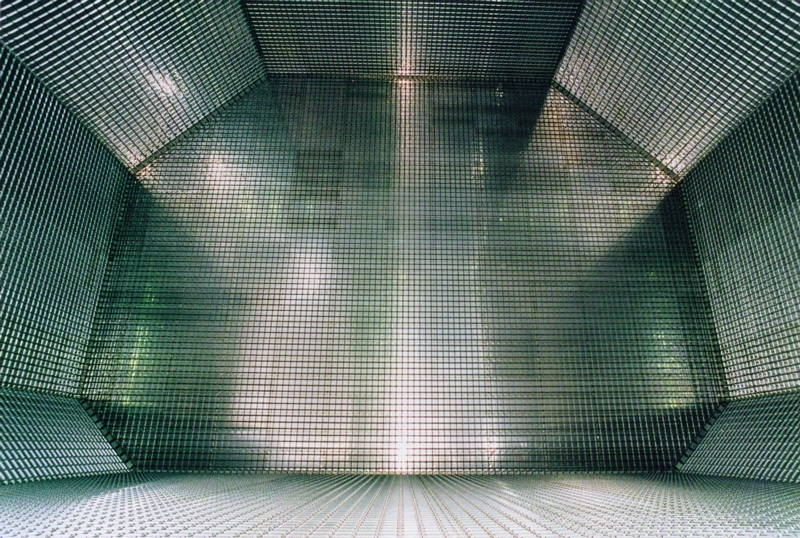
\includegraphics[width=\textwidth]{v5ch2-memb-tank-int}
\caption[Interior of a LNG ship tanker]{Interior of a LNG ship tanker. %A typical tank from one of two potential vendors is made of four 40,000~m$^3$ compartments, 35~m high by 45~m wide. 
The tank shown is 24~m high by 35~m wide with interior grid-like corrugations on a 0.34-m pitch.  By comparison, a  single LAr-FD cryostat is %18887~m$^3$, 
14~m high by 15.1~m wide.}
\label{fig:memb-tank-int}
\end{figure}

\begin{figure}[htbp]
\centering
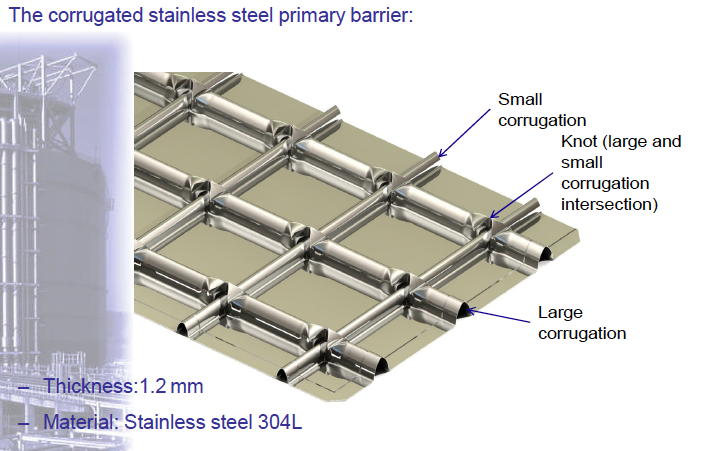
\includegraphics[width=.7\textwidth]{v5ch2-prim-barrier}
\caption[Primary membrane section]{Primary membrane section (courtesy GTT)}
\label{fig:prim-barrier}
\end{figure}

The advantages offered by the membrane design relative to a self-supporting cryostat are:
\begin{itemize}
%\item Lower cost due largely to the relative simplicity of a single cryogenic volume
\item Efficient use of the underground cavern volume due to its direct attachment to the rock on floor and sides,
which reduces the civil construction costs for the project
\item Higher ratio of usable (fiducial) mass to total mass
\end{itemize}

Conceptual design studies and studies done by ARUP, USA \cite{docdb4314} indicate that the implementation strategy for the cryogenics system is independent of the cryostat design. During the conceptual design studies two membrane cryostat vendors have been identified.  Those vendors are GTT (Gaztransport \& Technigaz) and IHI (Ishikawajima-Harima Heavy Industries).  Each is technically capable of delivering a membrane cryostat that meets the design requirements for the LAr-FD.  To provide clarity, only one vendor is represented in this CDR (GST system from GTT); this is for informational purposes only and should not be construed as preferring GTT over IHI.  Nothing inherent in the IHI design changes the design approach. 
%ARUP has documented the two vendor products in their Fall 2011 report that updated previous designs specficially to the two-20-kT module design at the 800L. 

\section{Design Parameters}
\label{sec:cryo-cryosys-params}

The requirements and parameters for the cryostat and cryogenic system design are within the LAr-FD requirements documentation~\cite{lar-fd-req}~\cite{lar-fd-req-traceback}  and the parameter tables~\cite{lar-fd-params}, respectively. The overarching system requirements are to provide a high-purity, stable liquid argon environment for the TPC and to provide mechanical support for the TPC. 
For components that pass through the ullage (the vapor space above the LAr), no sources of reliquefaction may be present. Tables \ref{table:param-summ-LAr-FD} and 
\ref{table:cryo-reqs} offer a brief overview of parameters for a single cryostat of LAr-FD.

\begin{table}
\caption{Design parameters for one LAr-FD Cryostat}
\label{table:param-summ-LAr-FD}
 \begin{tabular}[htbp]{|l| p{8cm} |}
\hline 
\textbf{Parameter} &  \textbf{Value} \\
\hline
Total Volume: &  7075 m$^3$ \\
\hline
LAr Total Mass: & 9.2 kton \\
\hline
Inner Height of the Tank: & 14.0~m \\
\hline
Inner Width of the Tank: & 15.1~m \\
\hline
Inner Length of the Tank: & 33.5~m  \\
\hline
Insulation:&  Reinforced Polyurethane; 80~cm thick \\
\hline
Primary Membrane(GTT): & 1.2-mm thick type 304L stainless steel with corrugations on 340~mm $\times$ 503~mm rectangular pitch\\
\hline
Secondary Containment(GTT): &  $\approx$ 0.07-mm thick aluminum between fiberglass cloth; overall thickness is 0.8 mm located between insulation layers \\
\hline
Outer Concrete Layer: & 0.5~m thick, inner surface treated with a vapor barrier \\
\hline
LAr Temperature: & 89 $\pm$ 1~K \\
\hline
Depth of the Liquid (Liquid Head): & 13.0~m \\
\hline
Design Operating Pressure (Above Liquid):&  0.113 MPa \\
\hline
Design Operating Pressure (Bottom of Liquid):&  0.2217 MPa \\
\hline
Rated Pressure Capacity of Tank:& 0.52~MPa (calculated according to BS EN 14620)
(British-Adopted European Standard / 29-Dec-2006 / 60 pages ISBN: 0580497763) \\
\hline
\end{tabular} 
\end{table}

% BN Jan 20 2012 changed Table to reflect 4850L

\begin{table}
\caption{Summary of parameters for the 4850L membrane cryostat} 
\label{table:cryo-reqs}
\begin{tabular}[htbp]{| p{0.35\textwidth}|p{0.65\textwidth}|}
\hline 
\textbf{Property} & \textbf{Reference-Design Cryostat}\\
\hline
Personnel access to cavern & Ross Shaft\\
\hline
Equipment transport to cavern & Ross Shaft and Yates Shaft (long items)\\
\hline
Construction access to pit & From above highbay \\
\hline
Type of crane in cavern & mobile construction \\
\hline
Base slab & Reinfoced concrete \\
\hline
Side walls & Reinforced concrete \\
\hline
Heating system & Redundant / Replaceable Electric system \\
\hline
Roof & Pre-fabricated steel truss modules with lower steel plate \\
\hline
Vapor barrier & Polymeric on concrete surfaces / steel plate on roof  \\
\hline
Insulation / Secondary barrier / Membrane & GST system by GTT \\
\hline
TPC & Individual 2.3 $\times$ 6m frames lowered through 2m x 4m roof hatch. Assembled within cryostat and suspended by hangers passing through the roof. \\
\hline
LAr containment system & Full containment: Membrane / Secondary Barrier / Concrete Liner  \\
\hline
\end{tabular} 
\end{table}



\section{Cryostat Configuration}
\label{Sec:cryo-cryosys-cryostat}

\subsection{Sides and Bottom of Tank}

The membrane tank is a sealed container that relies on external support from the surrounding rock to resist the hydrostatic load of the contents. In order from innermost to outermost layers, the side walls of the membrane tank consist of the stainless-steel primary membrane; insulation; a secondary, thin aluminum 
membrane that contains the LAr in case of any leaks in the primary membrane; more insulation; a barrier to prevent water-vapor ingress to the cryostat; concrete; shotcrete and rock.  This ``in-ground'' tank arrangement (i.e., offering access only from the top) protects against possible cryogen leaks out of the tank --- there is no place for the cryogen to go because it is surrounded on all sides by rock. The membrane cryostat is considered a ``full containment" system in the LNG industry lexicon. The basic components of the membrane tank are illustrated in Figure~\ref{fig:composite-sys-install}.



\begin{figure}[htbp]
\centering
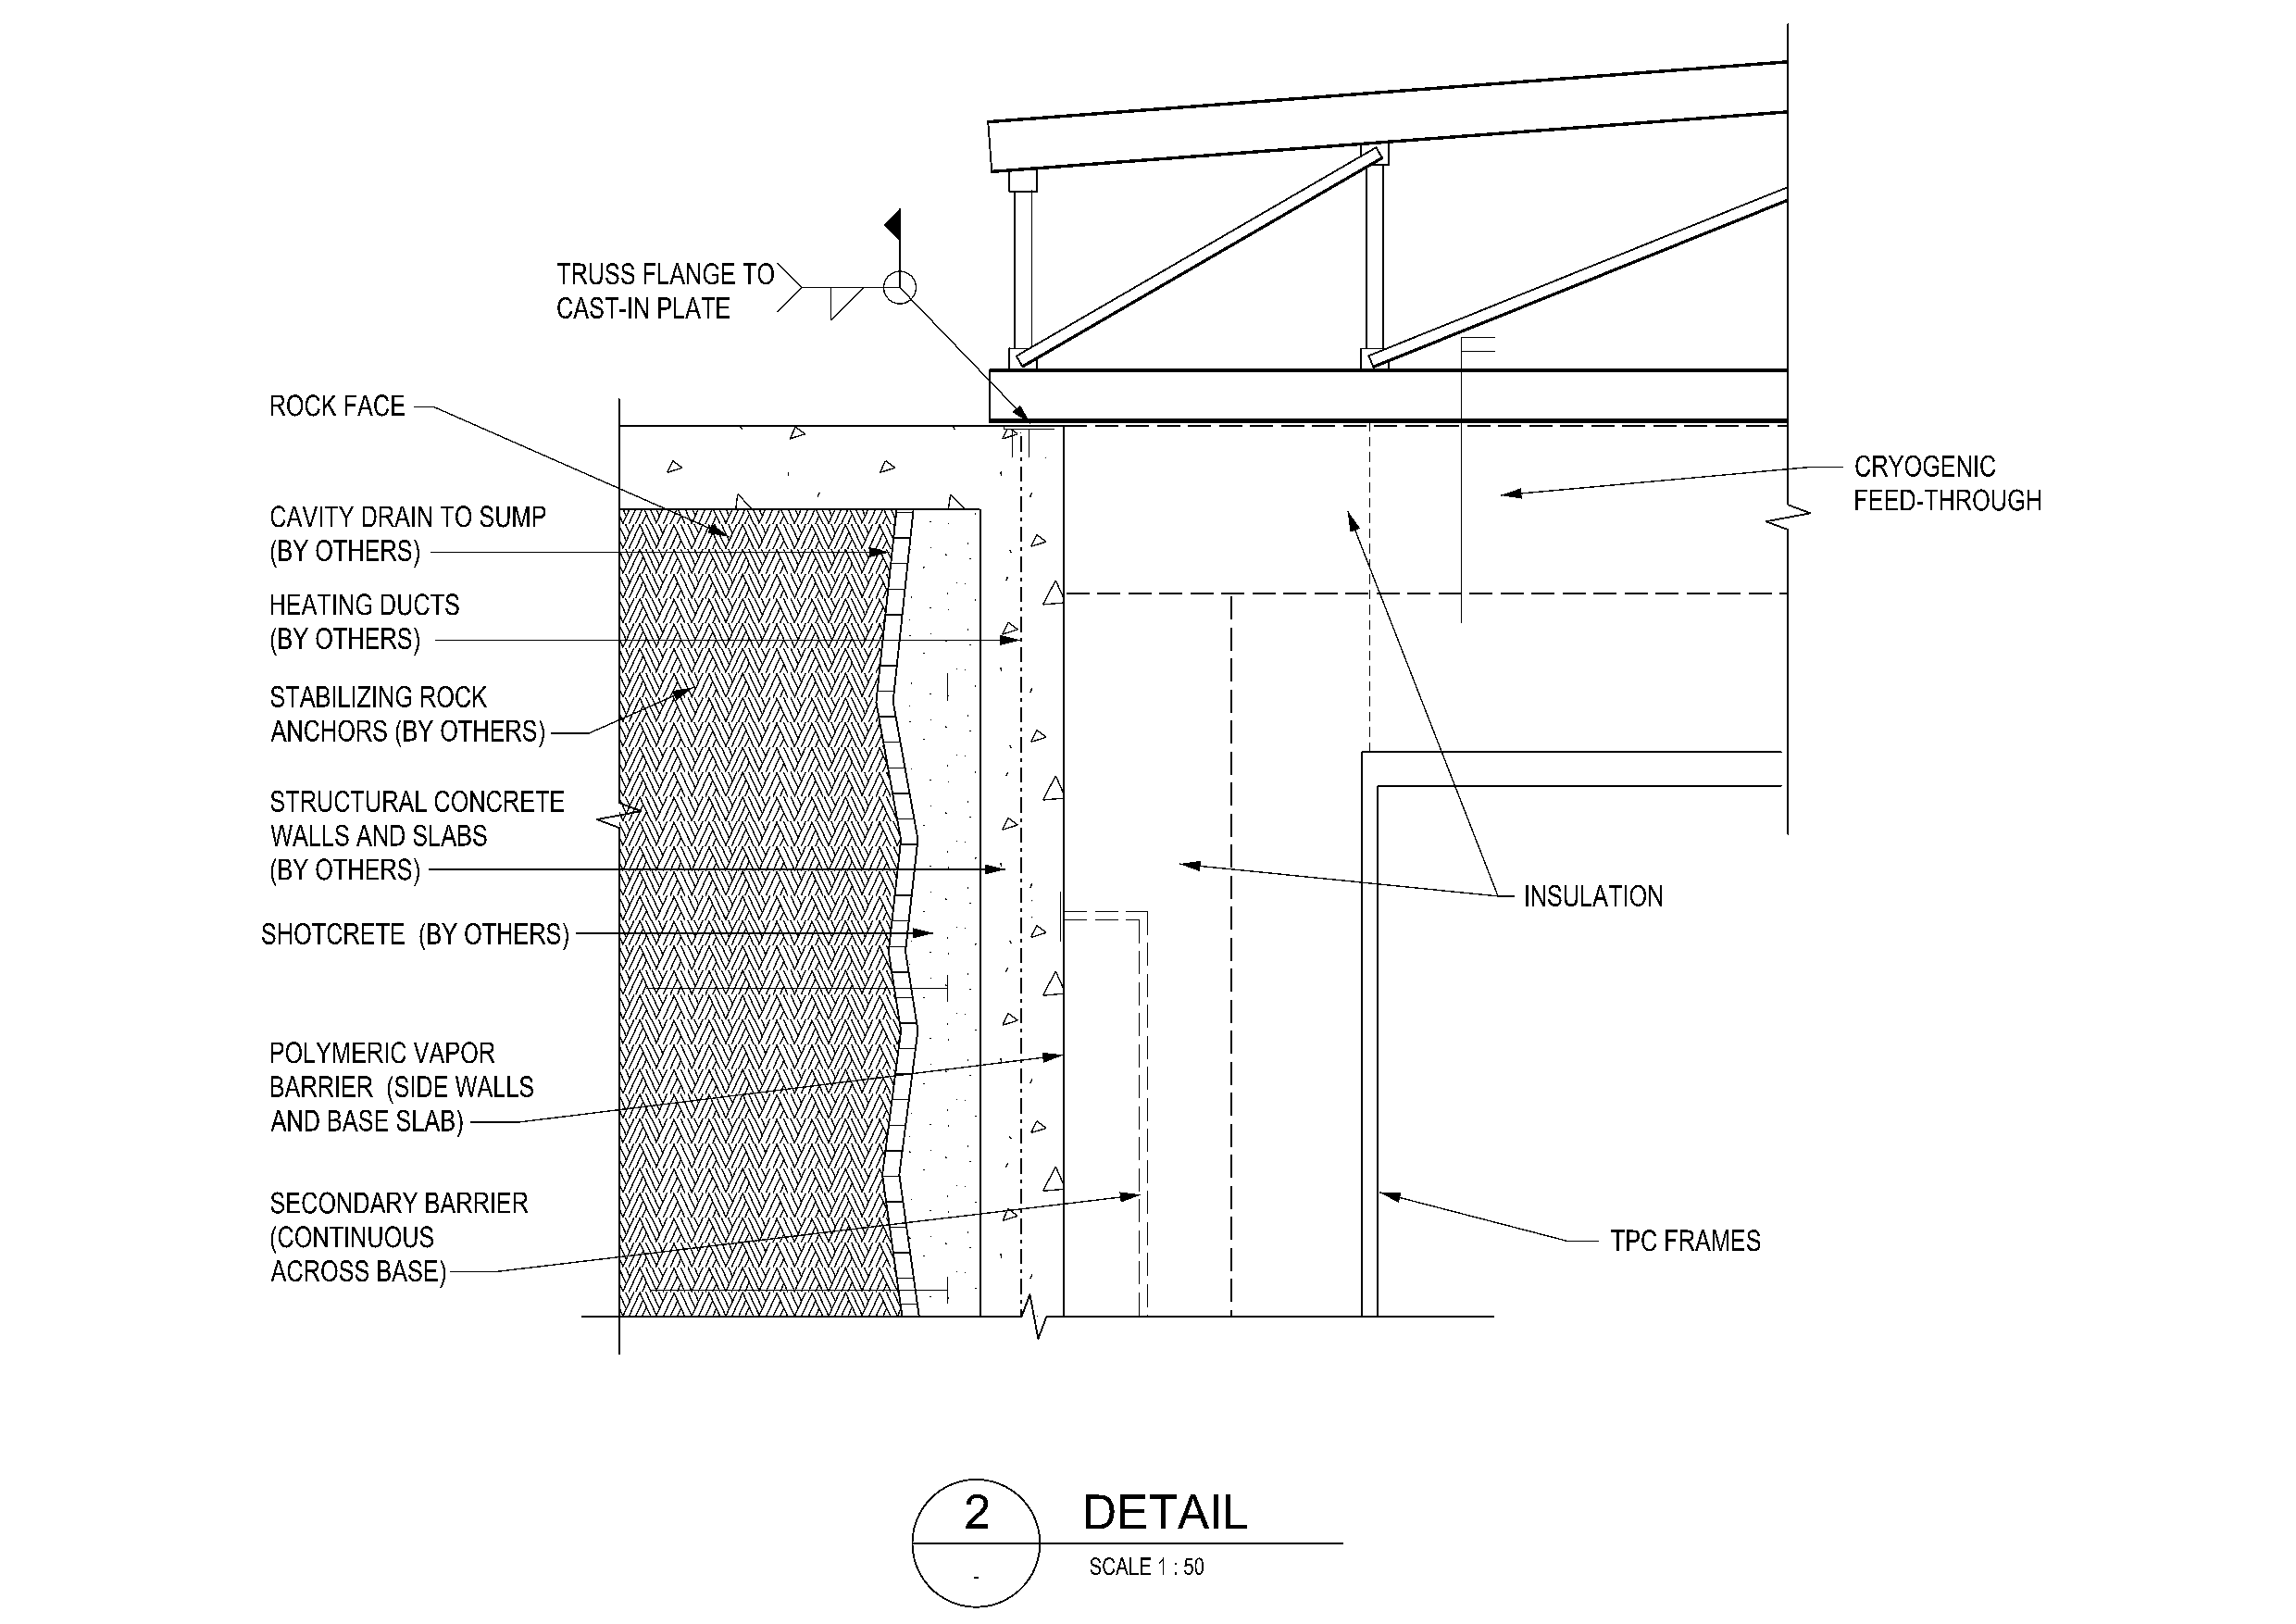
\includegraphics[width=\textwidth]{v5ch2-composite-sys-install-020612}
\caption{Composite system as installed for the LAr-FD reference design} 
\label{fig:composite-sys-install}
\end{figure}



\subsection{Concrete Liner and Vapor Barrier}
The formed concrete liner will be poured against the sides and bottom of the excavated rock pit. Conduits and heating elements will be embedded in the concrete liner to maintain rock temperatures above freezing to preclude any problems associated with freezing water and heaving as the rock temperature drops below the freezing point of water.  The embedded conduits are encased approximately midway in the concrete side walls, end walls and bottom floor slab as depicted in Figure~\ref{fig:endview-liner}.  The concrete liner and conduits are provided under the conventional facilities scope.  The heating elements are provided by LAr-FD scope.

\begin{figure}[htbp]
\centering
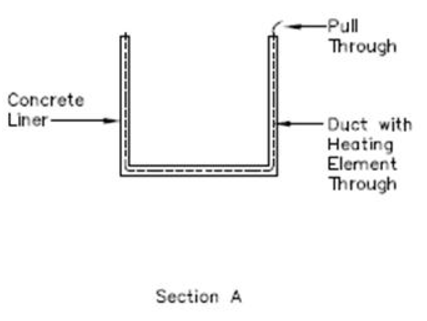
\includegraphics[width=.5\textwidth]{v5ch2-memb-heat-1}
\caption[End view of concrete liner showing embedded conduits for heating elements]{End view of concrete liner showing embedded conduits for heating elements (Courtesy Arup)}
\label{fig:endview-liner}
\end{figure}

A vapor barrier is required on all internal surfaces of the concrete liner (base slab, side walls, end walls) 
and the roof to prevent the ingress of any water vapor into the insulation space. If water vapor were permitted to migrate into the insulation space it could freeze and degrade the thermal performance of the insulation. The barrier must also reliably absorb the stresses and strains from all normal loading conditions. The selected vapor barrier material is a polymeric liner for the side and bottom surfaces.  This has been used extensively in onshore LNG tank applications.  The vapor barrier for the top will be solid steel plate welded together and to the underside of the roof truss.


\subsection{Insulation System and Secondary Membrane}
\label{subsec:insul-2nd-mem}

The membrane cryostat requires insulation applied to all internal surfaces of the concrete liner (base slab, 
side walls, end walls) and roof in order to control the heat ingress and hence the required refrigeration load. 
Choosing a reasonable, maximum insulation thickness of 0.8~m, and given an average conductivity 
coefficient for the insulation material of C $\approx$ 0.0283~W/m-K, the heat input from the surrounding rock 
is expected to be 13.7~kW per cryostat. %This is shown in Table~\ref{table:heat-load-calc}.  


% deleted \caption{Heat load calculation (Thickness = 1~m for all) }
% deleted \label{table:heat-load-calc}

The insulation material, a solid fiberglass foam, is manufactured in 1-m $\times$ 3-m composite panels. The panels will be laid out in a grid with 3-cm gaps between them (that will be filled with loose fiberglass) and fixed onto anchor bolts embedded into the concrete at $\sim$3-meter intervals. 
The composite panels contain an outer insulation layer, the secondary membrane and an inner insulation layer. After positioning adjacent composite panels and filling the 3-cm gap, the secondary membrane is spliced together by epoxying an additional layer of secondary membrane over the joint.  All seams are covered so that the secondary membrane is a continuous liner. A corner detail is shown in Figure~\ref{fig:vessel-corner}.


\begin{figure}[htbp]
\centering
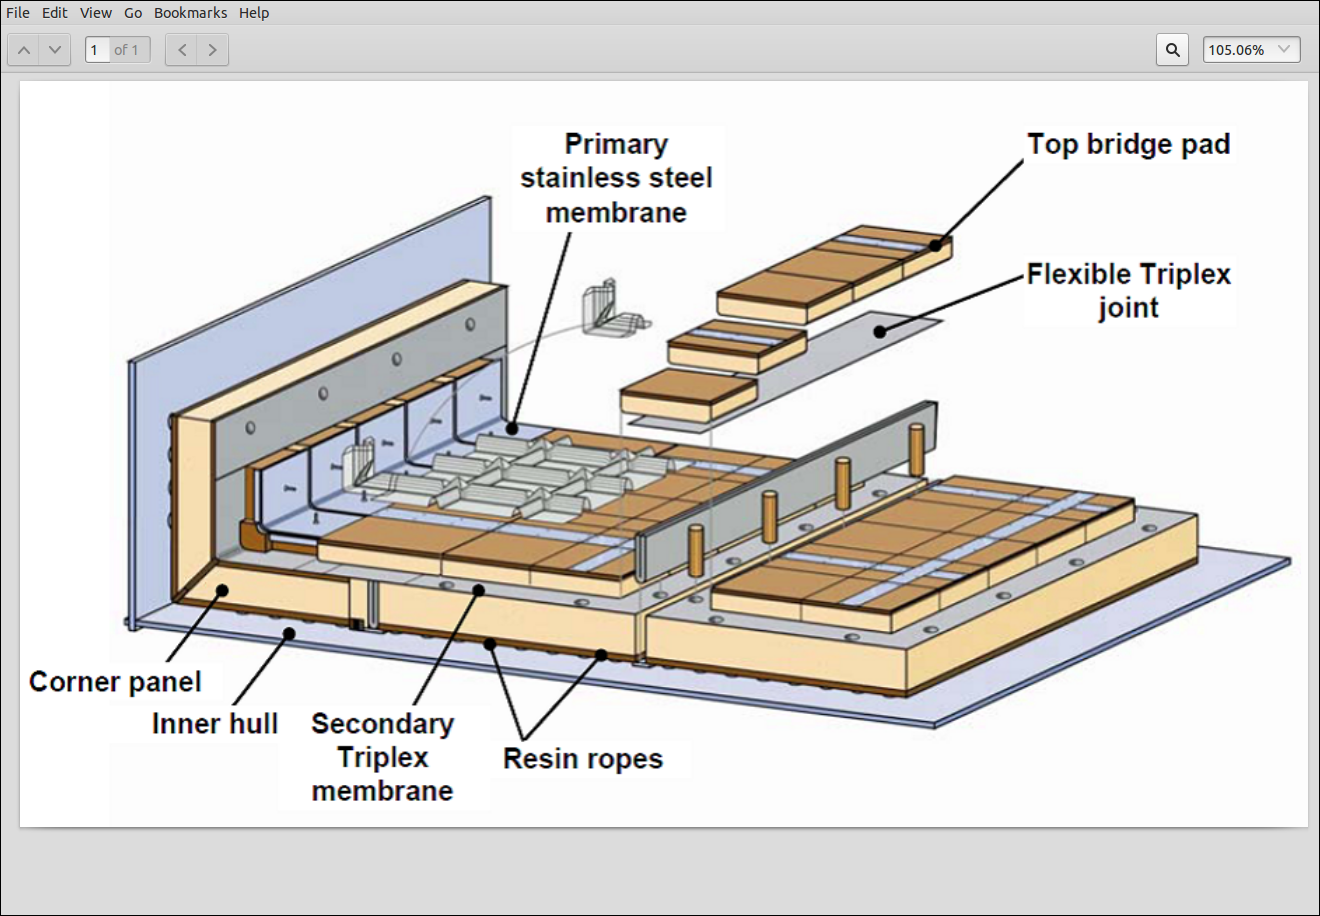
\includegraphics[width=.7\textwidth]{v5ch2-vessel-corner}
\caption{Membrane corner detail}
\label{fig:vessel-corner} %fig from email from russ 10/25
\end{figure}

The secondary membrane is comprised of a thin aluminum sheet and fiberglass cloth.  The fiberglass-aluminum-fiberglass composite is very durable and flexible with an overall thickness of $\sim$1~mm.  The secondary membrane is placed within the insulation space. It surrounds the internal tank on the bottom and sides, and it separates the insulation space into two distinct, leak-tight, inner and outer volumes. The outer insulation separates this membrane from the concrete.  
This sheet is connected to embedded metal plates in the vertical concrete wall at the upper edge of the tank. In the unlikely event of an internal leak from the cryostat's primary membrane into the inner insulation space, it will prevent the liquid cryogen from migrating all the way through to the concrete liner where it would degrade the insulation thermal performance and could possibly cause thermal stress cracks in the surrounding concrete. The liquid cryogen in the case of leakage through the inner (primary) membrane will be contained in the secondary membrane volume.  

\subsection{Tank Layers as Packaged Units}
Membrane tank vendors have a ``cryostat in a kit'' design that 
incorporates insulation and secondary barriers into packaged units. See Figure~\ref{fig:gst-composite}.  
Figure~\ref{fig:composite-sys-install} illustrates how these layers would be used in the LAr-FD reference design.

\begin{figure}[htbp]
\centering
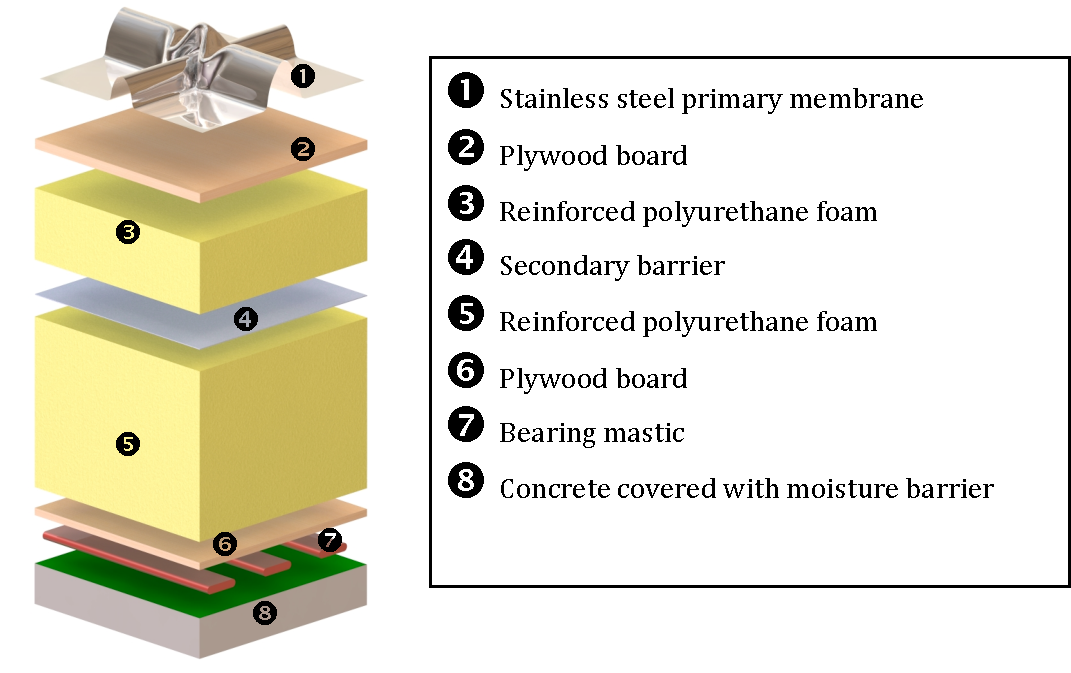
\includegraphics[width=0.7\textwidth]{v5ch2-gst-composite}
\caption{GST composite system from GTT}
\label{fig:gst-composite}
\end{figure}

\subsection{Top of Tank}

The stainless-steel primary membrane and the intermediate layers of insulation and water-vapor barrier continue across the top of the detector, providing a vapor-tight seal.  Note that no secondary membrane is used or required for the cryostat top. 
The cryostat roof is a steel truss structure that bridges the detector.  Stiffened steel plates hermetically welded to the underside of the truss form a flat vapor barrier surface onto which the roof insulation attaches directly; this is described more fully below. Fully fabricated roof trusses are placed across the roof with a 2.5-m spacing.  Field-fabricated truss members and steel plates are welded between the prefabricated trusses to connect the two prefabricated sections.  The roof is built up of alternating prefabricated and field-fabricated ``in-fill'' roof sections.  This configuration was selected during the screening process because it provides an efficient, gas-tight solution that can be readily constructed within the cavern space.

The truss structure rests on the top of the concrete wall as shown in Figure~\ref{fig:composite-sys-install} where a positive structural connection between the concrete and the truss is made to resist the internal upward force caused  by the slightly pressurized LAr in the cryostat.
The hydrostatic load of the LAr in the cryostat is carried by the floor and the side walls.  Everything else within the cryostat (TPC planes, electronics, sensors,
cryogenic- and gas-plumbing connections) is supported by the steel plates under the truss structure. All piping and electrical penetrations into the interior of the cryostat are made through this top plate to minimize the potential for leaks.

Studs are welded to the underside of the steel plates to bolt the insulation panels to the steel plates.  Insulation plugs are inserted into the bolt-access holes.  The primary membrane panels (also manufactured in smaller sheets) are first tack-welded then fully welded to complete the inner cryostat volume.  Feed-through ports as shown in Figure~\ref{fig:v5ch2-roof-nozzle} are located at regular intervals within the corrugation pattern of the primary membrane to accommodate TPC hangers, electrical and fiber-optic cables, and piping.
The roof truss will be anchored to the top of the poured-concrete liner walls to resist the uplift caused by internal tank overpressure (Figure~\ref{fig:roof-truss}).  The roof truss will be pre-fabricated off-site in $\sim$2~m wide, 
fully-welded modules and transported to the cavern as required by the installation schedule.

\begin{figure}[htbp]
\centering
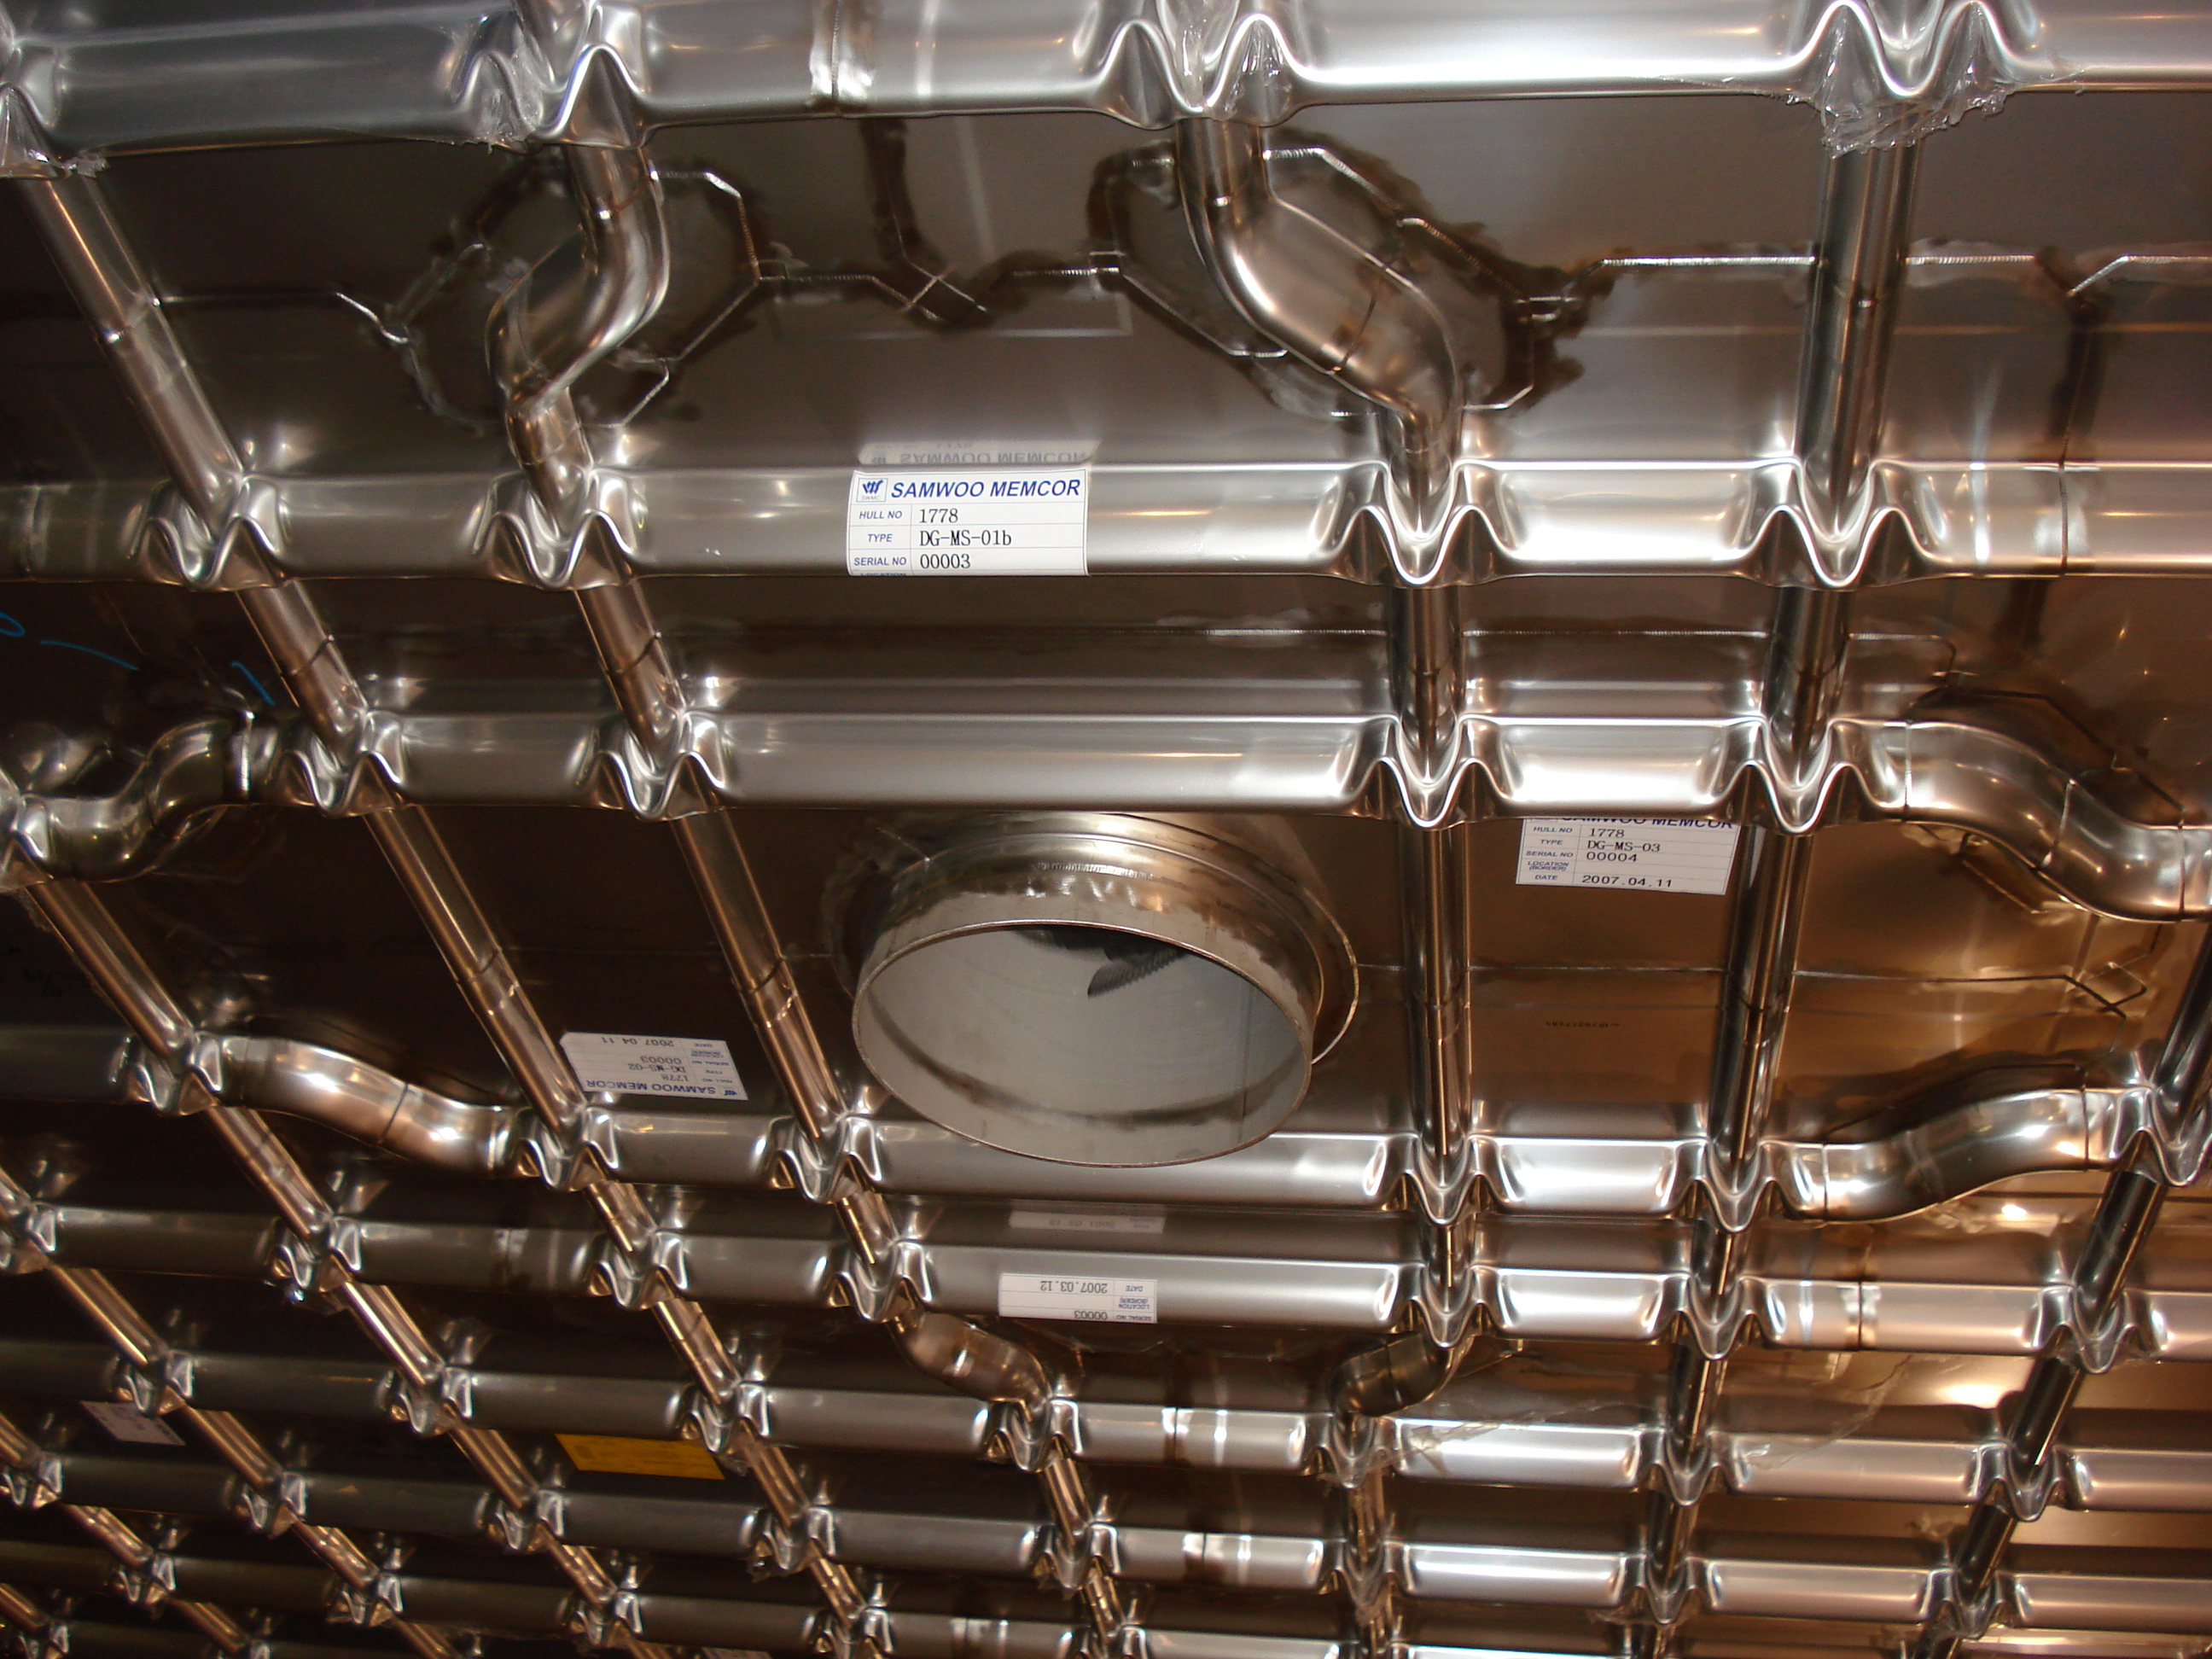
\includegraphics[width=0.6\textwidth]{v5ch2-roof-nozzle} 
\caption[Nozzle in roof membrane cryostat]{Nozzle in roof membrane cryostat (Figure courtesy GTT)}
\label{fig:v5ch2-roof-nozzle}
\end{figure}


%AH moved from under circulation
 The prefabricated steel roof-truss modules are relatively lightweight ($\sim$~8,000~kg each) and require only moderate crane capacity.  If the steel trusses need to be separated into smaller pre-fabricated 
units for transport to the 
%shallow or deeper 
underground site, assembly within the cavern space prior to installation is 
relatively straightforward. The truss construction is illustrated in Figure~\ref{fig:roof-truss}.

\begin{figure}[htbp]
\centering
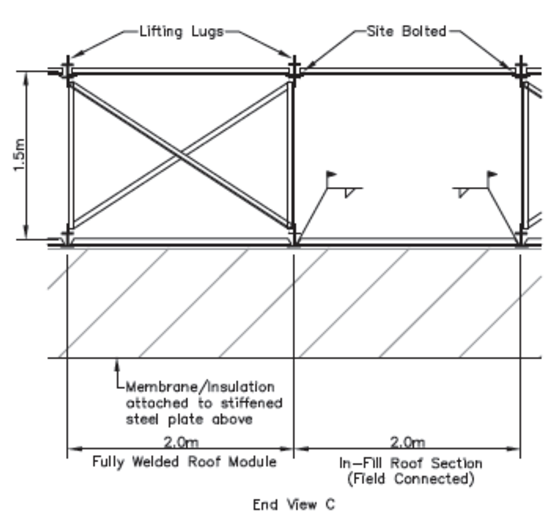
\includegraphics[width=0.5\textwidth]{v5ch2-roof-truss-2}
\caption[Roof truss structure]{Roof truss structure  (Courtesy Arup)}
\label{fig:roof-truss}
\end{figure}

Some equipment, such as monitoring instrumentation and pumps, will be installed within wells extending through the roof structure. All connections into the cryostat will be made via nozzles or penetrations above the maximum liquid level and 
mostly located on the roof of the cryostat.  See figure \ref{fig:v5ch2-roof-nozzle} for a typical roof-port penetration.  


\section{LAr Circulation and Temperature-Profile Modeling}
\label{sec:cryo-cryosys-temp}

The  liquid circulation in the LAr-FD cryostats has been modeled using computational fluid dynamics modeler software (ANSYS CFX).

A  field cage, described in Section~\ref{subsec:v5-tpc-chamber-fieldcage}, was modeled with half-inch slots cut every five inches, yielding a 10\% porosity.  Standard insulation thermal conductivity  of 0.0283~W/m-K was used to model the heat flux into the LAr. 
and used an exterior temperature of 278~K and an internal temperature of 87.15~K.  The temperature stability requirement on LAr-FD is $\pm$1~K.   The model  in Figures~\ref{fig:LAr-velocity} and ~\ref{fig:LAr-temperature} clearly identifies convective currents flowing through the entire liquid bath with the highest velocities $< 0.034$~m/s, and a temperature gradient much less than  0.1~K across the entire fluid body.  This 
indicates conformity with LAr-FD requirements and parameters.

\begin{figure}[htbp]
\centering
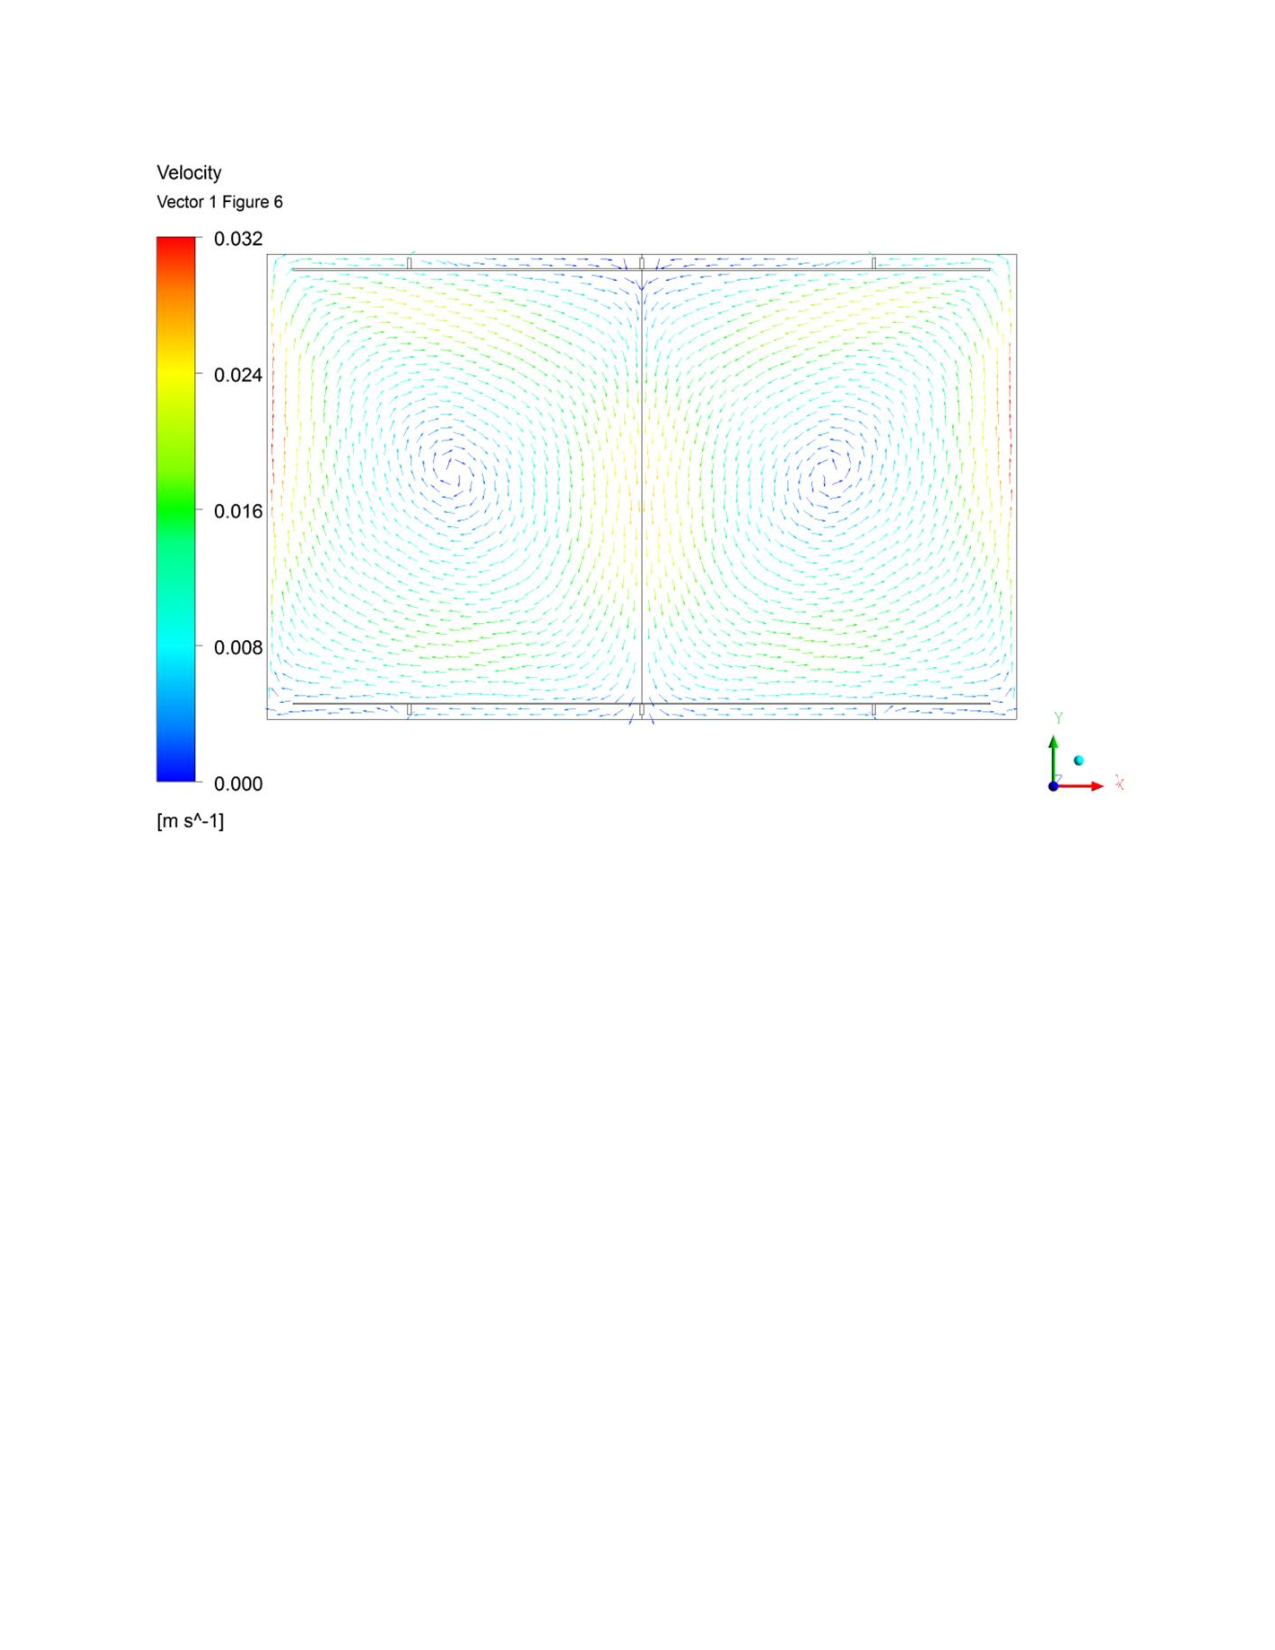
\includegraphics[width=.8\textwidth]{v5ch2-velocity}
\caption{LAr velocity profile} 
\label{fig:LAr-velocity}
%\end{figure}

%\begin{figure}[htbp]
\centering
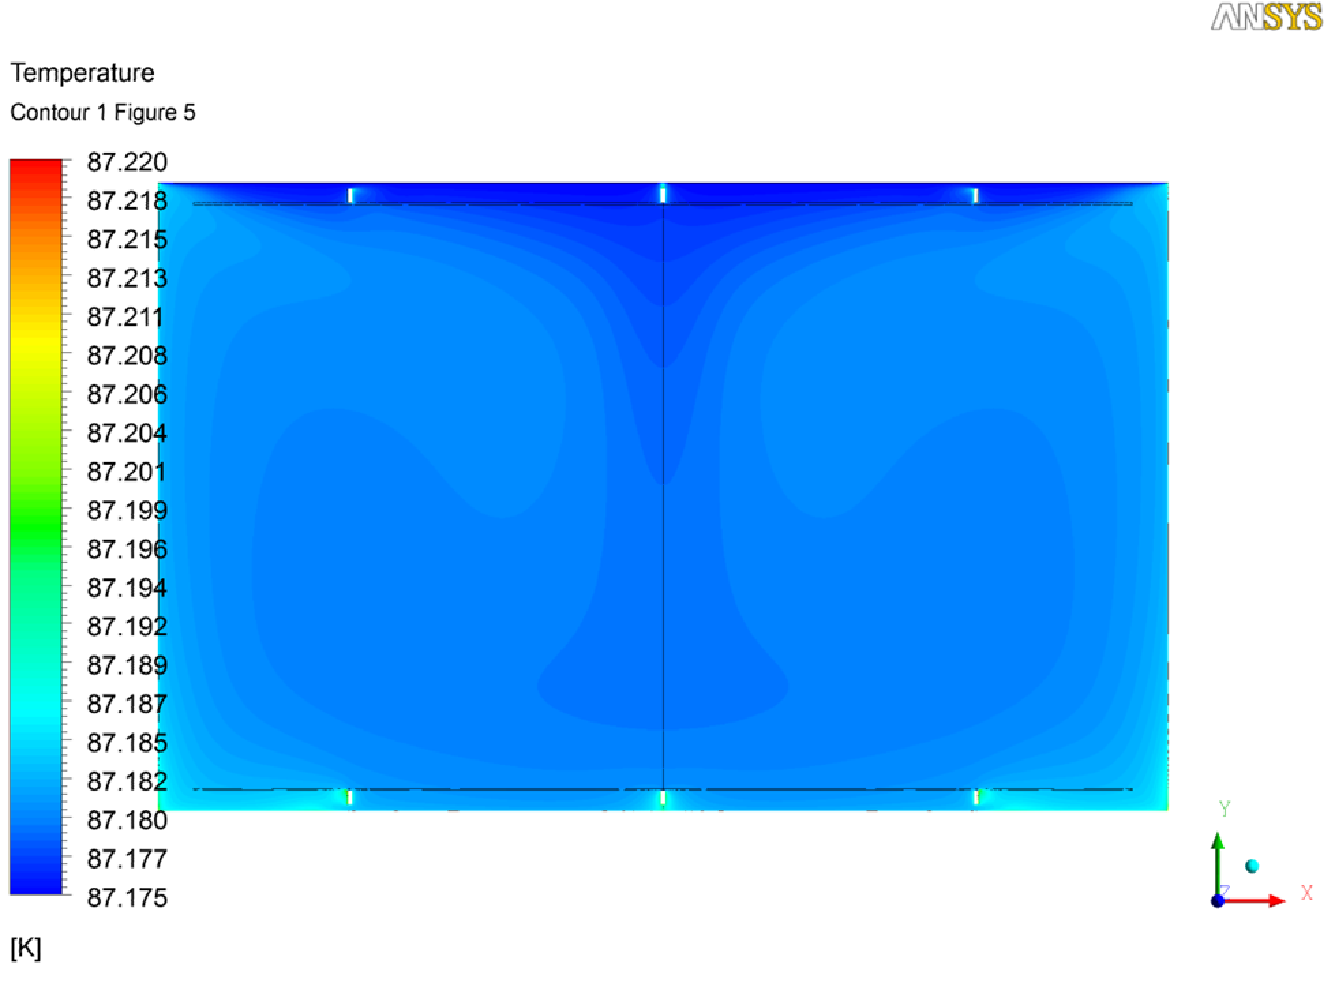
\includegraphics[width=0.8\textwidth]{v5ch2-temperature}
\caption{LAr temperature profile} 
\label{fig:LAr-temperature}
\end{figure}



\section{Leak Prevention}
\label{sec:cryo-cryosys-leak}

The primary membrane will be subjected to several leak tests and weld remediation, as necessary.  
All (100\%) of the welds will be tested by an Ammonia Colorimetric Leak Test (ASTM E1066-95) in which welds are painted with a reactive yellow paint before injecting gas with 25\% ammonia into the bottom insulation space of the tank.  Wherever the paint turns purple or blue, a leak is present. Both membrane cryostat manafucturers use this technique for certifying that a cryostat is leak-tight. Any and all leaks will be repaired. The test lasts a minimum of 20 hours and is sensitive enough to detect defects down to 0.003~mm in size and to a 10$^{-7}$ std-cm$^3$/s leak rate (equivalent leak at standard pressure and temperature, 1~atm and 273~K). 
Both membrane cryostat manafucturers use this technique for certifying that a cryostat is leak-tight.

%\subsection{Insulation Purge system}

To prevent infiltration of water-vapor or oxygen through microscopic membrane leaks (below detection level) the insulation spaces will be continuously purged to provide one volume exchange per day.  

The insulation space between the primary and 
secondary barriers will be maintained at 0.103~MPa, slightly above atmospheric pressure.  
This space will be monitored for changes that might indicate a leak from the primary membrane.  The outer insulation space will also be purged with argon at a slightly different pressure. The pressure gradient across the membrane walls will be maintained in the outward direction.  Pressure-control devices and relief valves will be installed on both insulation spaces to ensure that the pressures in those spaces do not exceed the operating pressure inside the tank.

The purge gas will be recirculated by a blower to a small purge gas dryer and reused as purge gas. 
The purge system is not safety-critical, and an outage of the blower would have only a minimal, short-term impact on operations~\cite{docdb4303}.

%%%%%%%%%%%%%%%%%%%%%%%%%%%%%%%%%%%%%%%%%%%%%%%%%%%%%%%%
\section{Cryogenic Systems Layout}
\label{sec:cryo-cryosys-layout}

Cryogenic systems are located on the surface and within the cavern. Figure~\ref{fig:eqp-at-surface}  illustrates the cryogenic systems layout. On the surface near the Ross shaft there will be a
cryogen receiving station. A 50-m$^3$
(69 tons liquid argon capacity) vertical liquid argon dewar
will have two LAr truck connections to allow for receipt of liquid argon deliveries for
the initial
filling period. The liquid argon dewar serves as a buffer volume to accept liquid argon at a pace
of about 5 liquid argon trailers (18 tons per trailer) per day during the fill period. An analyzer
rack with instruments to check water, nitrogen, and oxygen content of the trailers will also be
located in the vicinity. A large 280 kW vaporizer at the surface is used to vaporize the liquid
argon from the storage dewar prior to the argon gas being transferred by uninsulated piping
down the Ross shaft.

\begin{figure}[htbp]
\centering
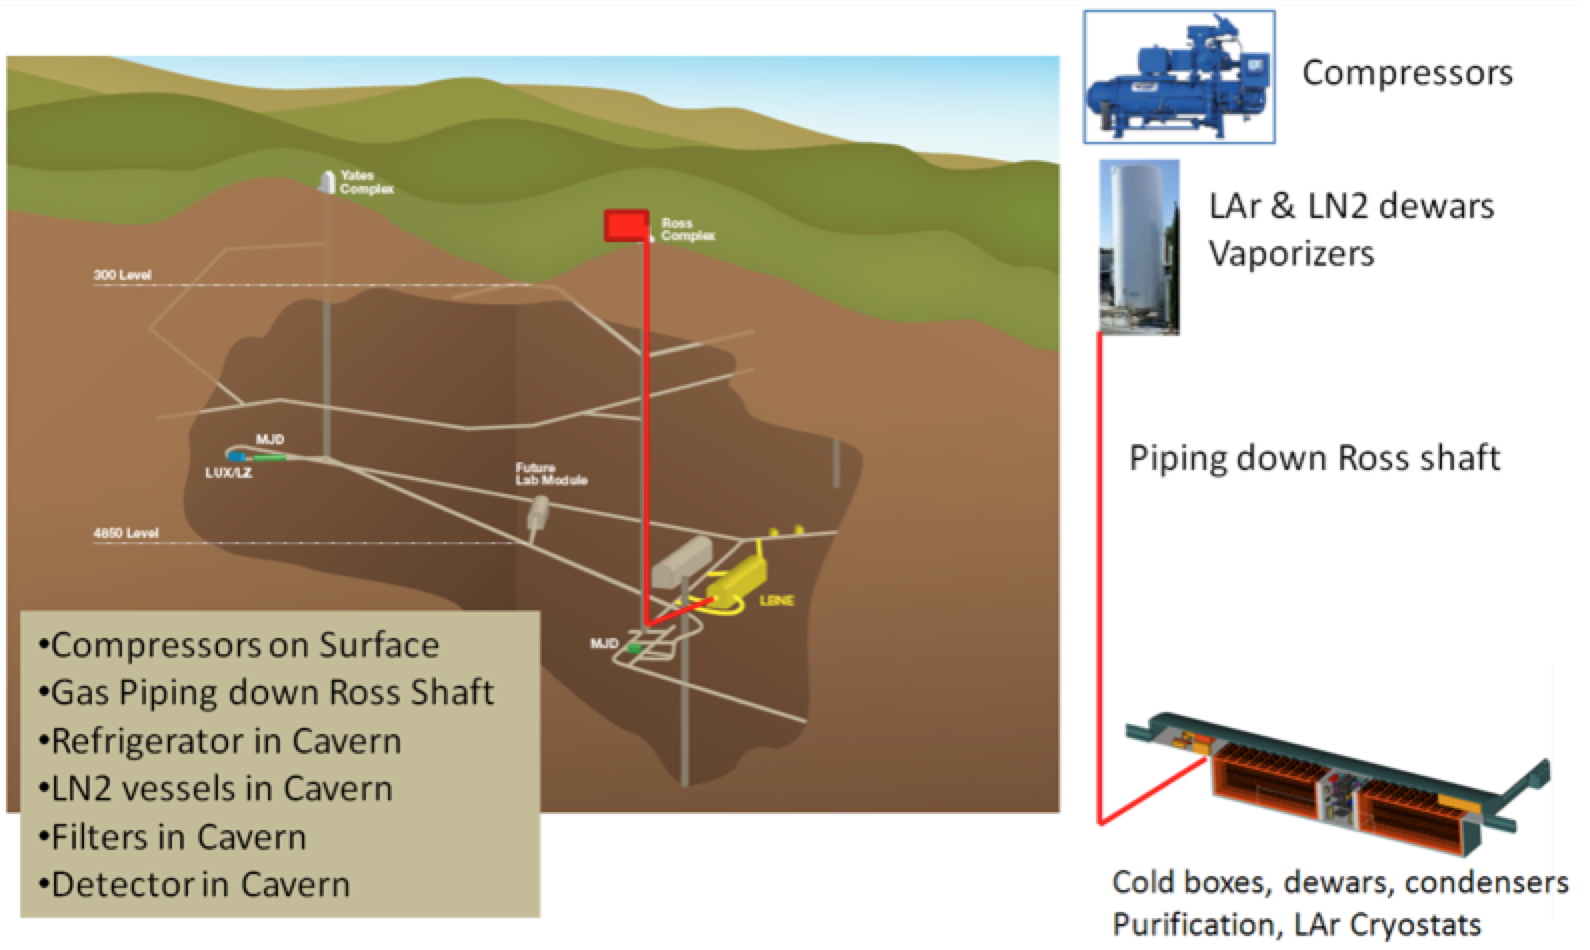
\includegraphics[width=\textwidth]{fd-cryosys-equip-loc-interim} 
\caption{Graphical illustrations showing major pieces of equipment and their location at the
surface, piping down the Ross shaft, and in the detector cavern}
\label{fig:eqp-at-surface}
\end{figure}


A 50-m$^3$ vertical liquid nitrogen dewar
and fill connection is located near the liquid argon dewar.
The nitrogen dewar is used to accept nitrogen deliveries for the initial charging and startup of
the nitrogen refrigerator. It is also used for pressure control of the liquid argon storage dewar.
A large vaporizer for the nitrogen circuit is located nearby to vaporize nitrogen to nitrogen gas
that is used as the feed for the compressors of the nitrogen refrigerator. Four compressors are
located in a compressor building located at the surface near the Ross shaft and cryogen
receiving area. The compressors require a closed loop water cooling circuit. The closed loop
water cooling circuit has recirculation pumps in the compressor building and an evaporative
cooling tower located outside near the
vaporizers. Only the compressors of the refrigerator are
located on the surface. The compressors discharge high pressure (1.1 MPa) nitrogen gas into
pipes that run down the Ross shaft. The compressors were chosen to be located on the surface
because the electrical power requirement and cooling requirement is much cheaper to provide
at the surface rather than at deep depth in the mine. Each compressor
is an 850 horsepower
machine running at 4160 volts. Four running compressors will require a total of
2.6 MW of electrical power at the surface.

The Ross shaft contains the vertical piping runs to connect the surface equipment with the
equipment in the cavern. The vertical piping runs are described
in Section~\ref{sec:cryo-cryosys-pipework-surface-cav}. 
Piping run consist of a
gas argon transfer line and the compressor suction and discharge lines. At the
bottom of the Ross shaft at the 4850 level, the piping exits the shaft and runs along a drift to
the detector cavern.

The detector cavern at 4850 level
contains the rest of the nitrogen refrigerator, liquid nitrogen
vessels, argon condensers, in-tank liquid argon recirculation pumps, and filtration equipment.
The cavern equipment is described in Section 2.8. The nitrogen
refrigerator equipment is
located at the end opposite the Ross shaft. Fresh ventilation air is supplied down the Ross
Shaft, enters the detector cavern and flows over the cryostats and then over the refrigerator
equipment before being exhausted out that e
nd of the detector cavern. The liquid nitrogen
vessels in the detector cavern are located in the crown of the cavern. A space for the
purification filters is opened up between the cryostats. It is known as the septum area. The 1.5
m thick concrete end
wall for each cryostat is separated by 15 meters of clear space to create
the septum area.

Each cryostat will have its own argon recondensers, argon-purifying equipment and
overpressure protection system.
Each set of systems is
placed on the septum side of the wall
closest to the cryostat it serves. Two 25-m$^3$/hr circulation pumps will be placed within each
membrane cryostat to circulate liquid from the bottom of the tank through the purifier.


\section{Pipework between Surface and Cavern}
\label{sec:cryo-cryosys-pipework-surface-cav}

The piping between the
surface and cavern is located in a utility chase down the Ross shaft.
See Figure~\ref{fig:framing-at-ross-piping}. The piping is single wall carbon steel pipe coated with a corrosion barrier. 
Table~\ref{table:pipelines} lists the piping and its duty and size. The frictional pressure drop for the supply pipes match
the pressure gained due to the static head
from elevation change. Piping will be all welded
construction. The nitrogen and argon being transferred in the Ross shaft piping will be at
ambient temperature, in the gas phase. Having gas phase only in the 1.5-km vertical piping is
an advantage over liquid transfer because the hydrostatic head for gas only piping is on order
0.05 MPa whereas for the liquid transfer it is 20 MPa. If liquid phase fluid was transferred it
would require on order
seven pressure reducing stations evenly spaced along the vertical drop.
Using liquid cryogenic delivery was considered, and in fact was the choice in the March 2012
CDR. However, the cost of providing the excavated spaces and pressure reducing stations
was costly as compared to using gas only transfer. For a liquid transfer option with pressure
reducing stations, the piping would need to be routed down the Oro Hondo ventilation shaft
which would need rehabilitation should that option be chosen. With gas only transfer to the
cavern, we can run straight piping down the Ross shaft. The drawback of gas only transfer is
that one must provide the liquid nitrogen refrigeration in the cavern to fill the cryostats by
liquid argon condensation. Filling each cryostat with liquid argon in a reasonable
period of time drives the refrigerator size and condenser sizing.

\begin{figure}[htbp]
\centering
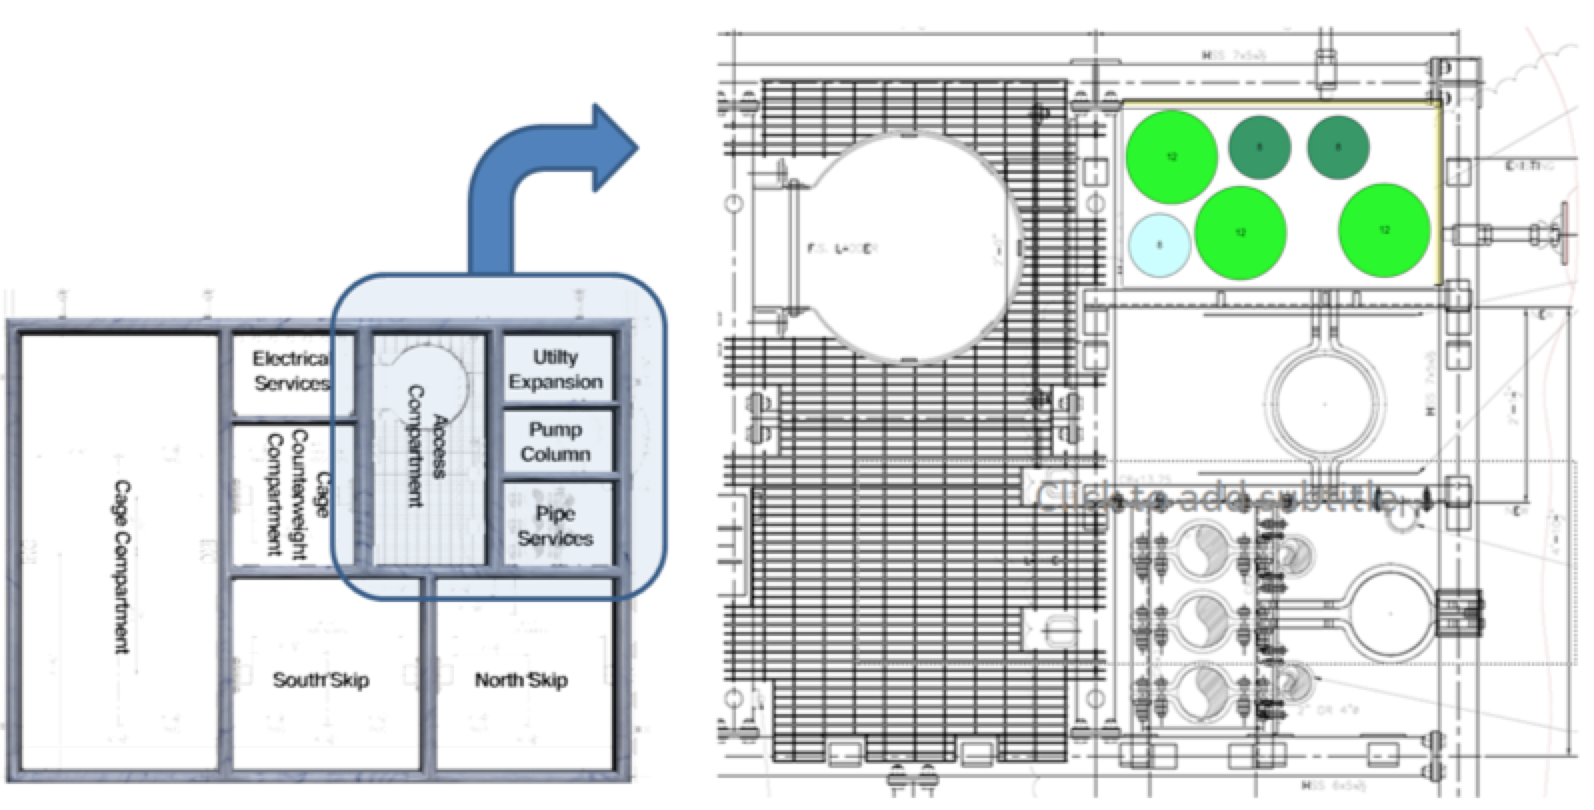
\includegraphics[width=\textwidth]{framing-ross-shaft-cryosys-piping.png} 
\caption{ The framing of the Ross shaft is shown on the left. The utility area in the upper
right corner contains the piping
associated with the cryogenic system}
\label{fig:framing-at-ross-piping}
\end{figure}

\begin{table}
\caption{Piping between surface and cavern; location, duty and required size}
\label{table:pipelines}
\begin{tabular}[htbp]{|p{0.35\textwidth}|p{0.3\textwidth}|p{0.12\textwidth}|p{0.12\textwidth}|}
\hline
{\bf Description} & {\bf Duty} & {\bf Size} & {\bf Fluid Pressure} \\
\hline
Argon transfer & During filling and emptying & 8'' sch. 40 &  0.24 MPa\\
\hline
N2 Compressor discharge & continuous & Two 8'' sch. 40 pipes & 1.14 MPa \\
\hline
N2 Compressor suction & continuous & Three 12'' sch. 40 pipes &  0.19 MPa at bottom, 0.11 MPa at top \\
\hline\end{tabular} 
\end{table}

A preliminary oxygen deficiency hazard (ODH) assessment for the piping in the Ross shaft has
been done. The mine fresh air ventilation is sizeable, 100,000 cfm supplied down the Ross and
Yates shafts. If any of the pipes for the cryogenic system ruptured in the shaft they would only
be able to reduce the oxygen content by a fraction to 20.5\%, thus not being an oxygen
deficiency concern.

\begin{figure}[htbp]
\centering
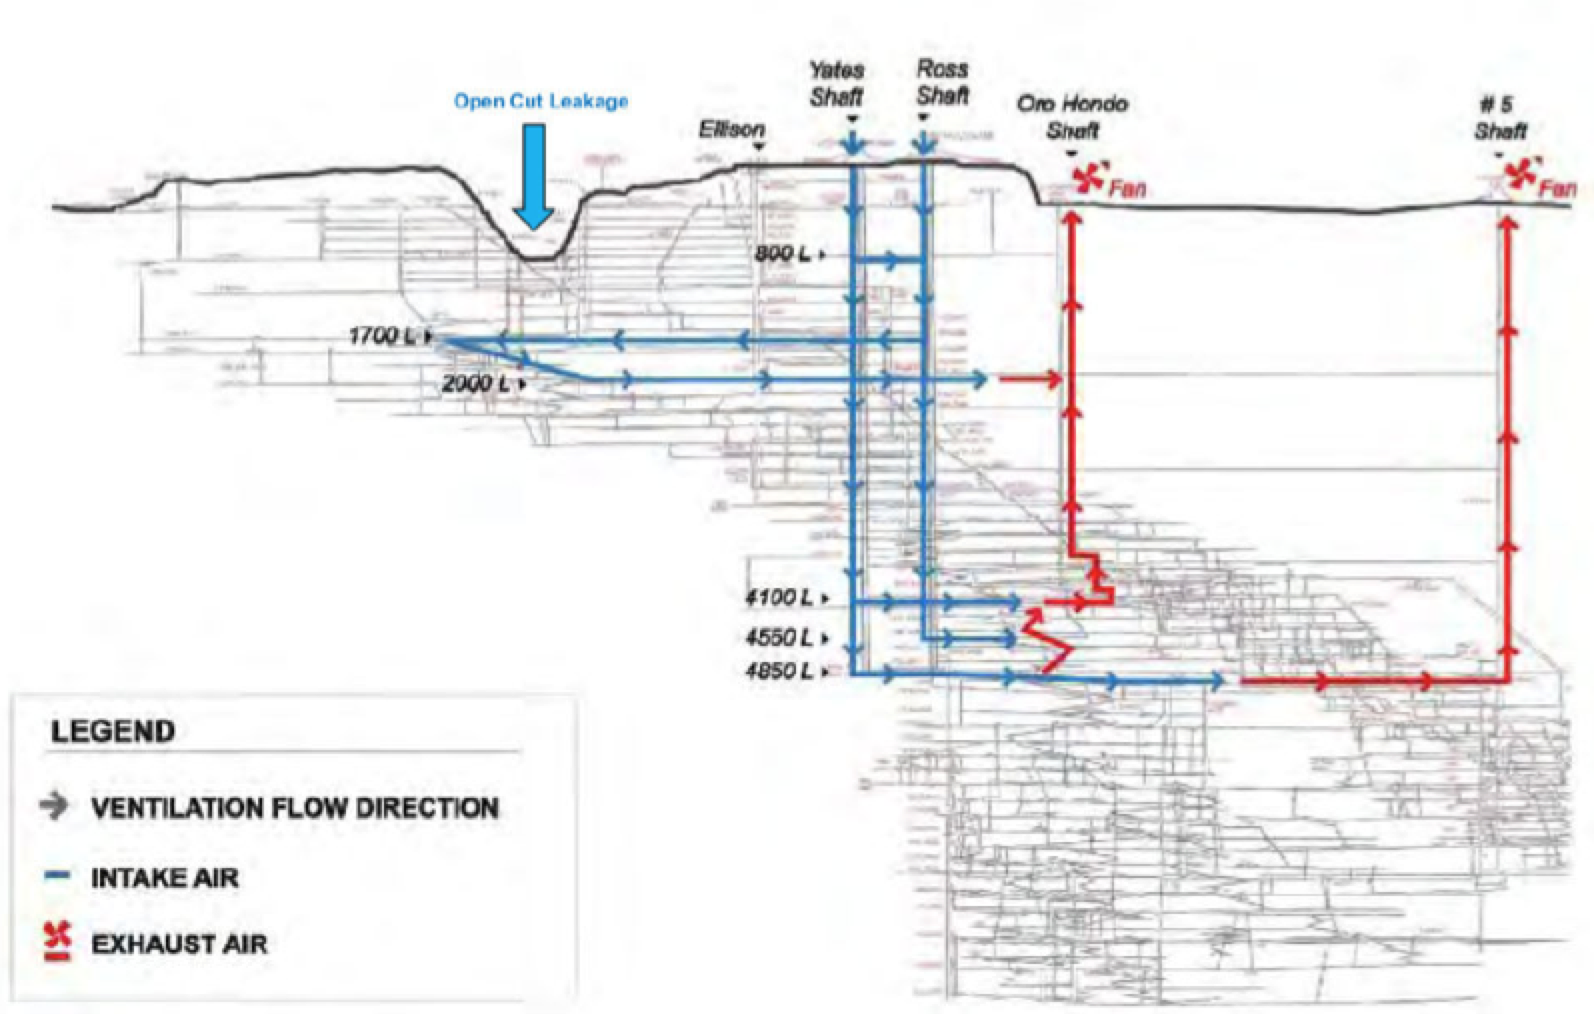
\includegraphics[width=\textwidth]{homestake-ventilation-paths.png} 
\caption{Homestake mine ventilation paths}
\label{fig:ventilation-paths}
\end{figure}


\section{Equipment in the Cavern}
\label{sec:cryo-cryosys-equip-cavern}

There are four independent 85 kW nitrogen refrigerators in the cavern. The nitrogen
refrigerator heat exchangers and expander sets are located at the east end of the detector hall.
The heat exchangers (1.2 m diameter $\times$ 9.1 m long) will be in a horizontal orientation in order to
fit them within the cavern. The liquid nitrogen produced by the refrigerators is stored in
eight horizontal 12.5-m$^3$ (1.2 m diameter $\times$ 11 m long) liquid nitrogen vessels that are mounted in the
crown space of the cavern over the refrigerator heat exchangers. These liquid nitrogen vessels
in turn feed the argon condensers that are connected to the cryostat. The returning nitrogen
gas from the condensers is routed through the refrigerator heat exchangers and warmed to
ambient temperature. The nitrogen gas is then boosted by four 120 kW compressors located in
the cavern to 0.19 MPa and returned up the nitrogen suction piping in the Ross shaft.

Three argon condensers (0.61 m diameter $\times$ 1.9 m long) for each cryostat are located at the
septum end of the cryostat. The full power of the argon condensers is used during the initial
filling phase of the cryostats to fill the cryostat by condensation of the gas argon transferred
down the Ross shaft. The fill process is expected to take 9.5 months for the first cryostat and
11.6 months for the second. Additional information about the filling process is described in
Section~\ref{sec:cryo-cryosys-proc}.  

\begin{editornote}
  Editor's Note:  Filling times in preceding sentences refer to filling two 17-kton modules.
\end{editornote}


Purification filters are located in a septum space between the cryostats as shown in Figure~\ref{fig:det-cavern-purif}. The filters (2.2 m
diameter $\times$ 4.5 m high) contain dual media, a molecular sieve for removal of water and a copper
coated catalyst media for oxygen removal. There is one gas filter that is used during the argon
filling phase and one liquid filter for each cryostat for a total of three. Associated with the
filters, there will be regeneration equipment such as heaters, gas blowers, and a hydrogen
generator also located in the septum area. 

\begin{figure}[htbp]
\centering
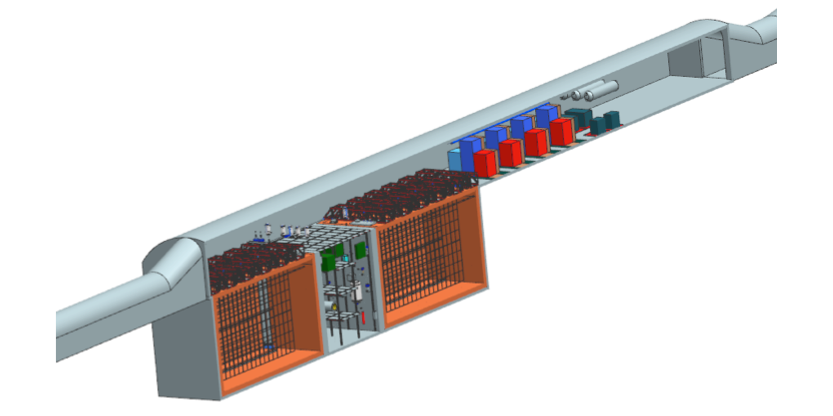
\includegraphics[width=\textwidth]{larfd-from-2794-slide9.png} 
\caption{Isometric view of the detector cavern showing purification equipment in a septum
space between the detector cryostats and refrigerator equipment at one end}
\label{fig:det-cavern-purif}
\end{figure}


\section{Cryogenic System Processes}
\label{sec:cryo-crysys-proc}
%added by russ 10/6
The functionality of the cryogenic system is
shown in Figure~\ref{fig:v5ch2-LAr-FD-block-diagram-2014}. This diagram shows
the interconnectivity between major functions of the cryogenic system. The major piping
connections can be seen in Figure~\ref{fig:v5ch2-LAr-FD-cryo-process-2014}. The major functions serving the
cryostat are cryogen supply for cool down and fill, gas
filtration, condensing, liquid filtration and circulation, argon-purity analysis, and argon condensing. The methods presented in this section are motivated by
experience from other LAr TPC cryogenic systems such as ICARUS and LAPD.

\subsection{Cryostat Inital Purge and Cool-down}

After cryostat construction and following installation of all scientific equipment, the cryostat
will be cleaned, purged and cooled. Construction procedures leading up to this point will
ensure that the completed cryostat does not cont ain debris and is free of all loose material that may contaminate the LAr.

\subsubsection{Initial Purge}

Argon piping will be isolated, evacuated to less than 0.1 mbar absolute pressure and backfilled
with high-purity argon gas. This cycle will be repeated several times to reduce contamination
levels to the ppm level in the piping. The reference-design choice for removing air from the
membrane cryostat will be to flow/piston-purge argon, introducing the heavy argon gas at the
bottom of the tank and removing the exhaust at the top. The bottom field cage (part of the
TPC), serves an additional role as a flow diffuser during the initial
purge. A matrix of small holes in the field cage will provide a uniform flow, approximately
10-mm diameter at a 50-mm pitch. 

The flow velocity of the advancing argon-gas volume will be set to 1.2 meters/hour. This is twice the diffusion rate of the air downward into the advancing argon so that the advancing pure argon-gas wave front will displace the air rather than just dilute it. A
2D ANSYS model of the purge process shows that after 20 hours of purge time and 1.5 volume changes, the air concentration will be reduced to less than 1\%. At 40 hours of elapsed time and three volume
changes, the purge process is complete with residual air reduced to a few ppm. This
simulation includes a representation of the perforated field cage at the top and bottom of the
detector and heat sources due to the readout electronics. The cathode
planes are modeled as non-porous plates although they will actually be constructed of stainless-steel
mesh.

The computational fluid dynamics (CFD) model of the purge process has been verified with
purge tests in an instrumented 1-m-diameter by 2-m-tall cylinder. Recognizing that obtaining
the required purity levels by the flow-purging method needs to be clearly demonstrated, a
Liquid Argon Purity Demonstrator (LAPD) project was undertaken
at Fermilab. The LAPD is a right-cylindrical vessel, 3 m in diameter and 3 m tall. LAPD took gas-sampling measurements
at varying heights and times during the purge process. Experimental measurements taken by
the Liquid Argon Purity Demonstrator (LAPD) have verified the previous modeling of this
purge process. During the first operation of LAPD, the vessel
needed nine volume changes to reach single-digit contamination levels
(ppm by volume) for oxygen, water and nitrogen. Following
the purge, the LAPD vessel was cooled down and filled with LAr.
On September 30, 2011, LAPD leaders presented initial results of this purge process in which
purity levels of less than 100 ppt oxygen-equivalent were achieved.
A second period of operation in FY13 has confirmed this approach yet again. The
purge method works and it minimizes the risk to LBNE that an evacuable vessel will be
required. This test will be repeated with a 35-ton membrane cryostat
prototype.

\begin{figure}[htbp]
\centering
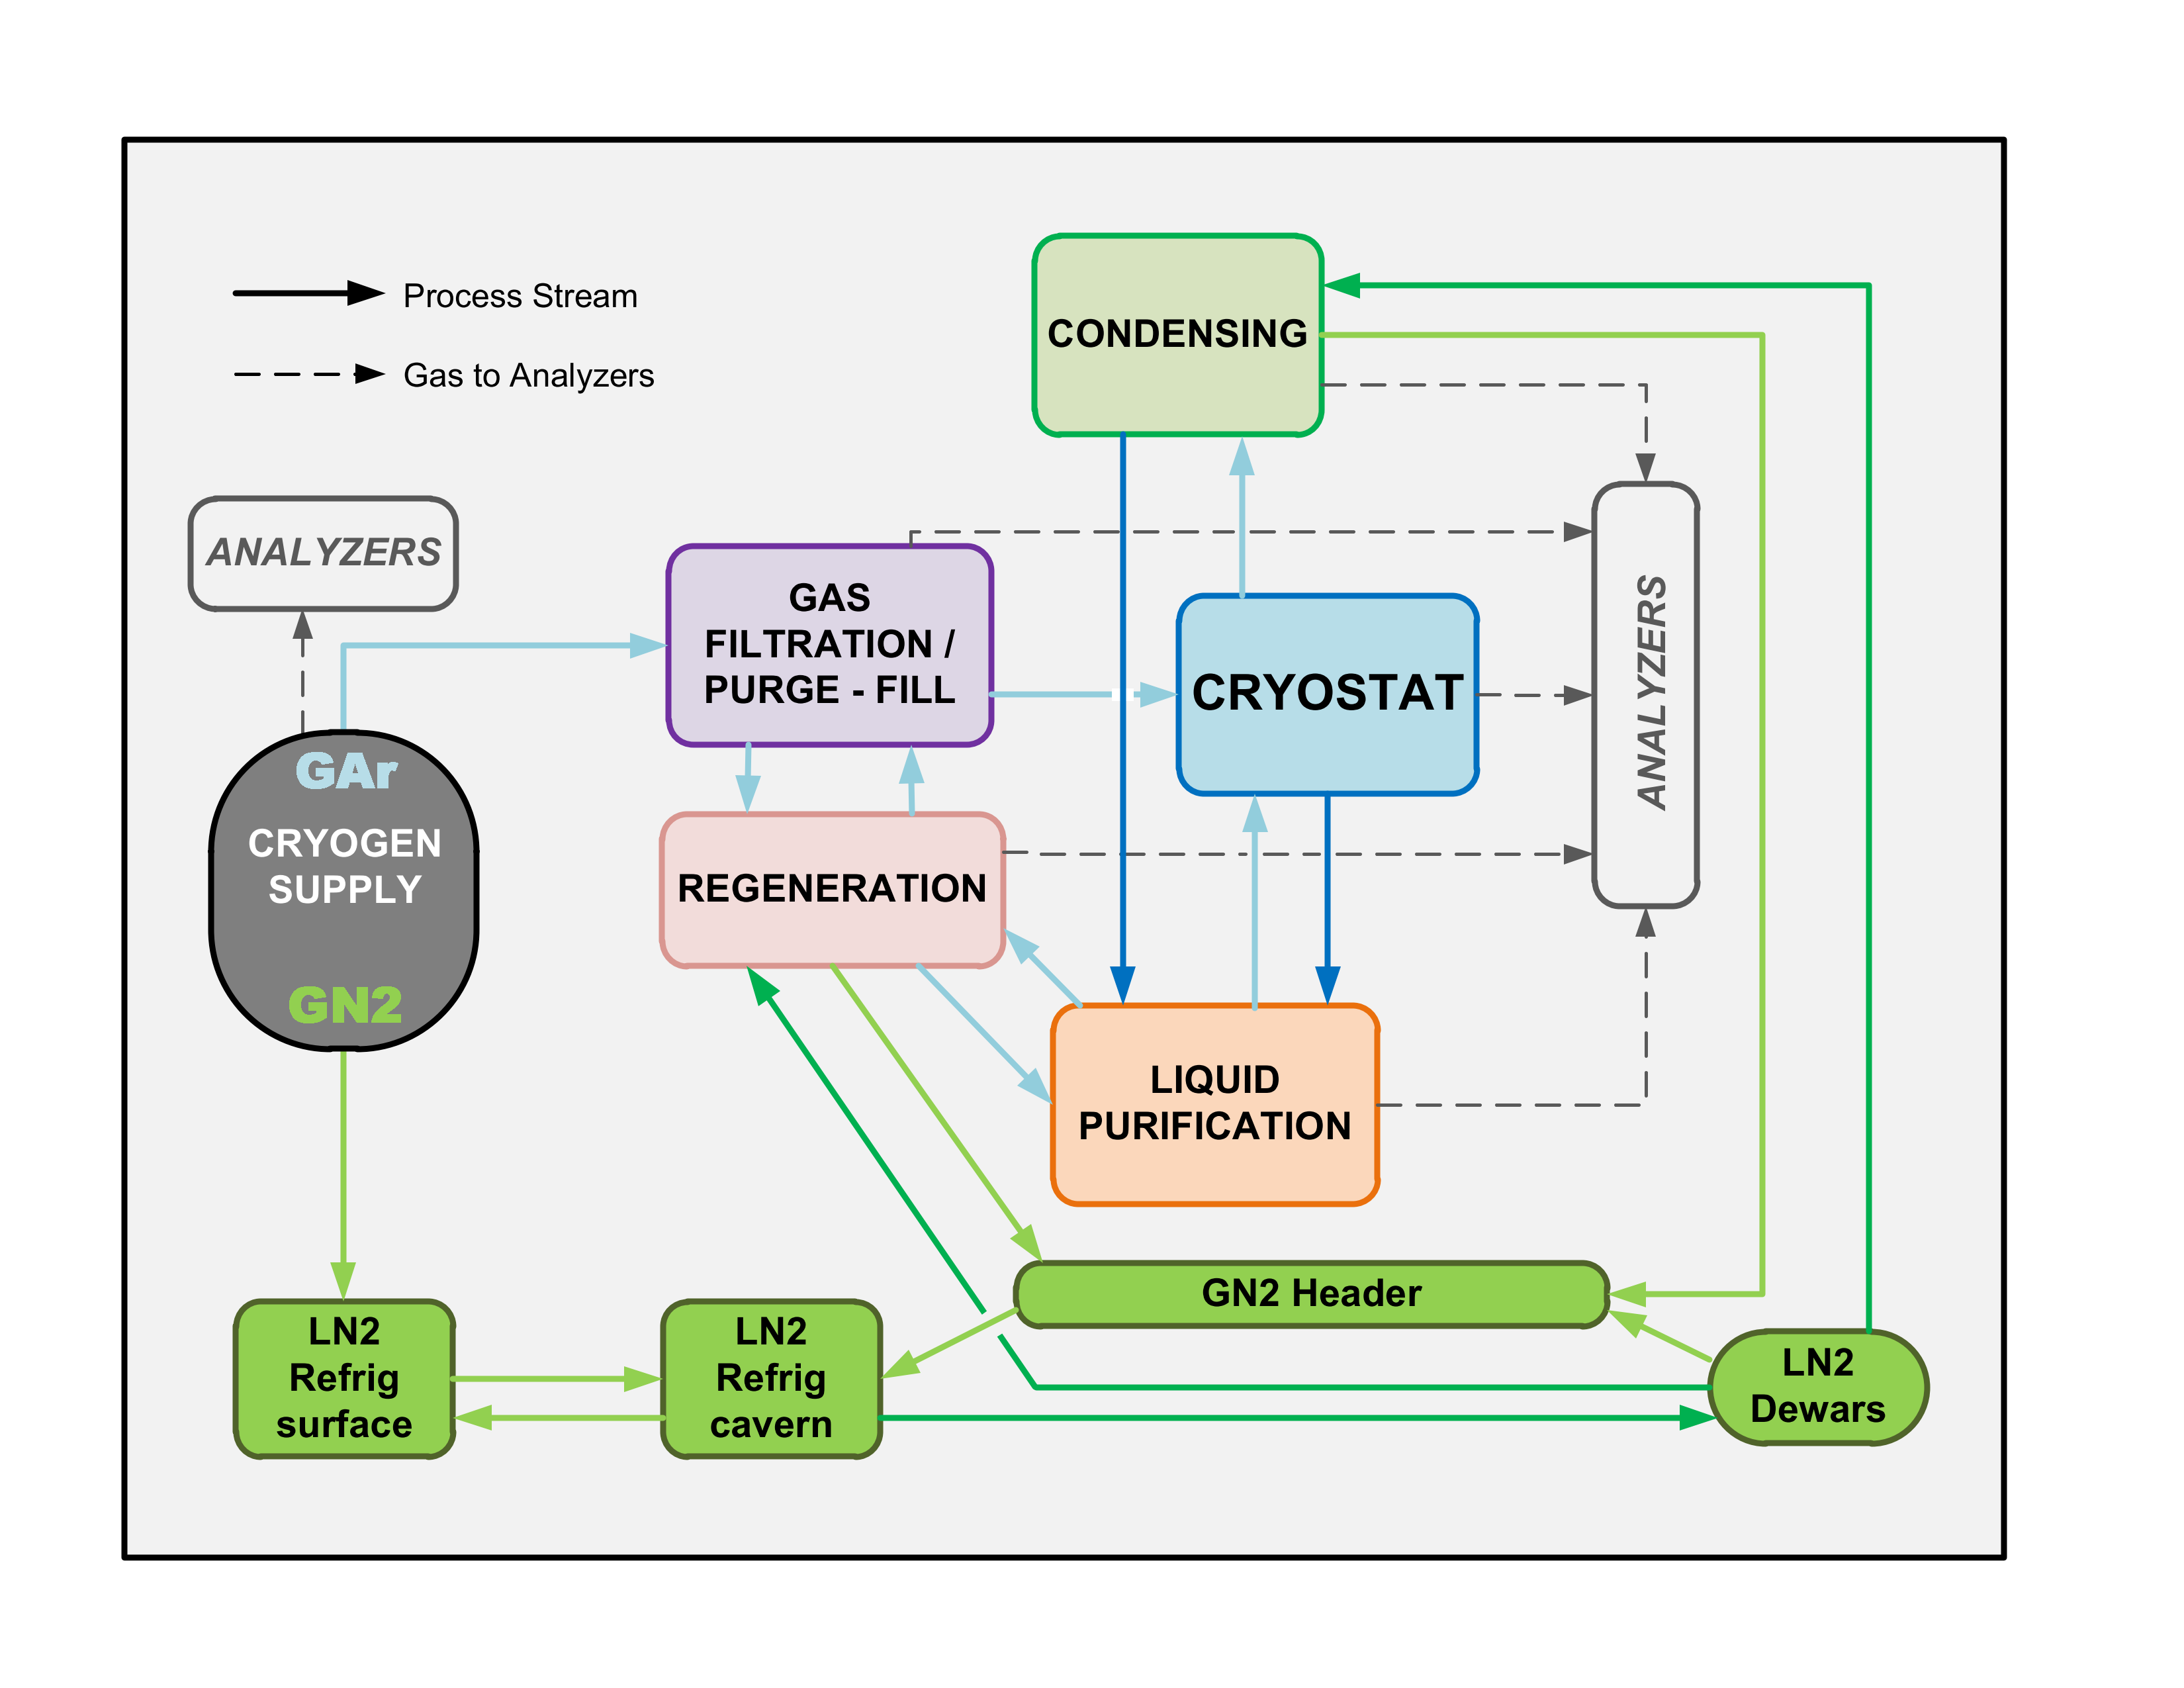
\includegraphics[width=\textwidth]{cryosys-functions.png} 
\caption{Cryogenic system functions}
\label{fig:v5ch2-LAr-FD-block-diagram-2014}
\end{figure}

\begin{figure}[htbp]
\centering
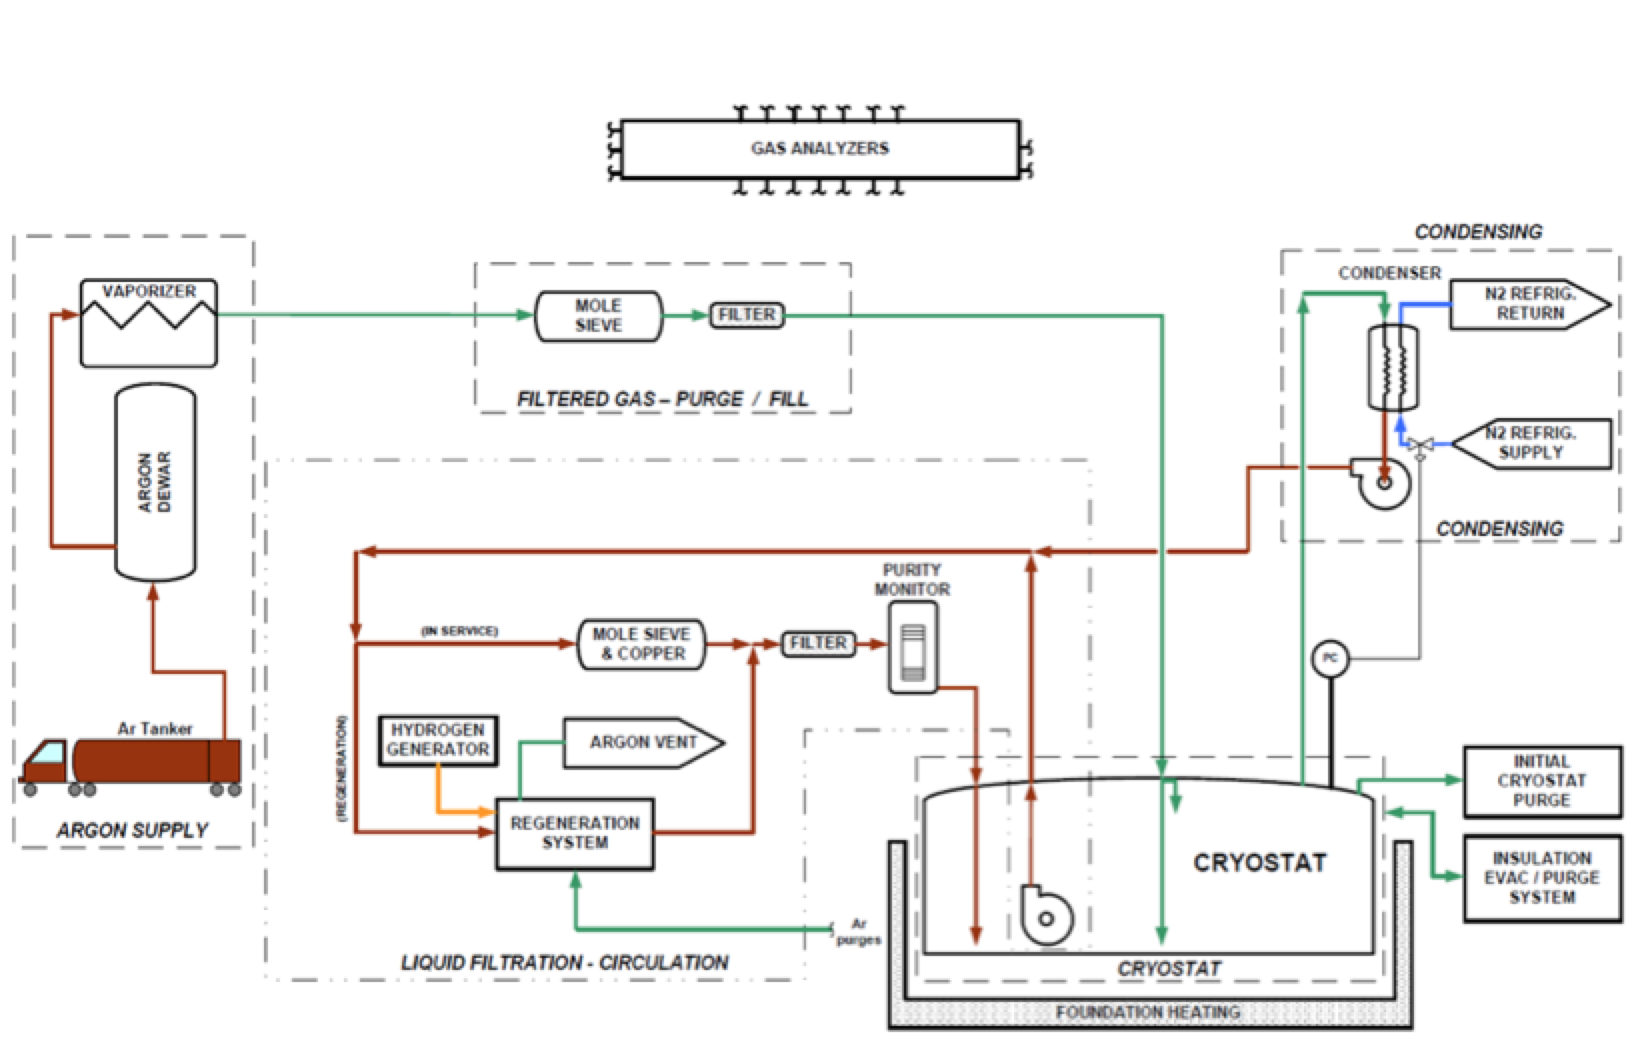
\includegraphics[scale=0.5,angle=90]{cryosys-flow.png} 
\caption{Cryogenic system block flow diagram}
\label{fig:v5ch2-LAr-FD-cryo-process-2014}
\end{figure}


% The elements of the plan and their applicability to LAr-FD are described in Chapter~\ref{ch:randd}.  BN didn't think this fit for techical report 10/06/11

\subsubsection{Water Removal via Gas Flow}

Water and oxygen will continue to be removed from the system for several days following the
initial purge. Flowing gas will be used at the same rate, however at this stage the gas will
be filtered and recirculated. Each cryostat contains five tons of FR4
circuit-board material and a
smaller inventory of plastic-jacketed power and signal cables. These somewhat porous
materials may contain as much as 0.5\% water by weight. Water-vapor outgassing from these
materials will be entrained in the gas flow exiting
the top of the cryostat and will be removed
from the gas stream by filters. Adsorbed water will also be removed from the metallic inner
surfaces of the cryostat and piping system. Water deep within porous materials will remain;
this is not a problem since
the water diffusion rate in FR4 at room temperature is already quite low (0.3~$\mu m^2 /s$) and the FR4 assemblies are relatively thick (1~cm).

\subsubsection{Alternative Water-Removal Method: Evacuation}

The traditional method for removing water and oxygen from LArTPCs is to evacuate the tank to $\sim$10$^{-4}$~mbar  and then backfill it with pure argon gas. Although the primary membrane of the reference-design cryostat is not a vacuum vessel, it is possible to evacuate it.  A membrane-cryostat vendor reports that evacuation of  the insulation spaces (external to the primary membrane) is normally done during the construction and leak-checking phases.  A vacuum pressure of less than 200~mbar absolute in the insulation spaces has so far been achieved.  As long as the pressure-differential direction across the walls is kept outward, it is possible to reduce the internal membrane-tank volume to these pressures as well.  

\subsubsection{Initial Cool-Down}

Purified LAr will be distributed near
the bottom of the cryostat to cool down the cryostat in a controlled spray.
(A design is being tested in the 35 ton prototype which is to become
operational in fall 2013). The boil-off gas will flow through the volume of the cryostat, then
routed to the recondenser and liquid-filtration system. Simulation
has shown that the liquid cool-down method can
be controlled to stay within the available recondenser capacity. The required cooling rate
is determined by the maximum stress that detector components can
tolerate. For example, the 150-$\mu$m APA wires will cool much more rapidly than the APA frames.
A mass flow control system with temperature-monitoring system will be used to control the
temperature difference across the cryostat. The exact temperature difference required is yet to
be determined; it will be based on input from the cryostat designer and the requirements of
the TPC components and structure.

\subsubsection{Initial Purge and Cool-Down Design Features}

Internal piping is positioned within the cryostat to support the purge and cool-down procedure.  Heavy argon vapor, which is a result of cooling down the membrane bottom with liquid, will promote purging after it rises from the base of the cryostat and is vented from the roof level.  The LAr-supply pipework will have nozzles spaced along its length to 
 distribute equal liquid-delivery flow rates across the bottom of the cryostat.  The flow nozzles will be directed downward or to the side so that the injection velocity will not cause local vertical gas plumes or turbulent mixing but rather will spread across the bottom of the tank and produce a stable, upwardly advancing argon wave front. The vertical velocity of 1.2~m/hr for the gas purge includes a contingency for some level of turbulent mixing. 

Main gas returns, used for pressure control, will be distributed along the cryostat roof.  All nozzles and dead-end (stagnant) volumes located at the top of the cryostat will have gas-exhaust lines for the initial purge and for continuous sweep-purge of those volumes during normal operations.  
The sweep-purge during the initial stage of purging will be vented outside of the cavern.  After all but trace amounts of air have been expelled, the gas returns will be routed to the recondensers before being returned to the cryostat.  When cool-down to 120~K is complete (and during steady state operations), the gas returns will be sent to the recondenser to be liquefied by heat exchange with a liquid nitrogen stream.  The recondensed liquid will be filtered and sent back to the cryostat to complete the cool-down operation.
All purge gas will be contained and either vented outside of the cavern at a remote location, or recondensed and reused. 

\subsection{Liquid Argon Receipt}

Each five-kton fiducial mass LAr detector module will hold an inventory of 9.2~kton of liquid argon.  Initial purge operations are expected to consume and exhaust about 0.25~kton per module.  Considering that some product will also be lost in transit, approximately 20~kton of LAr will need to be procured to fill the initial 10-kton detector.  Planning the logistics and supply of LAr to the facility requires consideration of the following issues:

\begin{itemize}
\item  total capacity of commercial air-separation plants within freight distance of the facility (the peak delivery potential)
\item extent of boil-off that will occur in transit
\item  number of vehicle movements required and their impact on the local community
\item costs and benefits associated with stockpiling LAr at the facility ahead of commencing the purge, cool-down and fill procedure
\item provision of a temporary air-separation plant at the facility to generate liquid argon
\item  availability and cost associated with the delivery of high-purity LAr as opposed to lower-quality, commercial-grade argon combined with on-site, coarse purification
\end{itemize}

Total argon production in the United States is currently approximately 3.6~kton per day.  Argon is normally co-produced along with large volumes 
of oxygen, so any project that requires large oxygen quantities may also spur additional argon production, enhancing the
supply capacity.  A 2013-2018 market-forecast report by the Freedonia group~\cite{freedonia} indicates that the demand for argon will increase at a rate of 3.4\% per year whereas the demand for oxygen will increase 4.8\%.  

The standard grade specification for argon is a minimum purity of 99.995\%, allowing a maximum concentration of 5.0~ppm for O$_2$ and 10.5~ppm for H$_{2}$O.  This is designated as Grade 4.5 in the gas-supply industry.  Requiring higher-purity product would significantly reduce the volume of product available to the experiment, increasing cost and pushing out the schedule.  
Therefore, standard product will be procured from multiple vendors.  

The most efficient mode of argon delivery is 
over-the-road tank truck with a maximum capacity of 18.7~metric ton (MT).  The expected number of such deliveries needed is 510 over nine and one-half months to fill one cryostat (the second cryostat will take >11 months to fill due to reduced cooling power after one detector is full and pure). 
Rail delivery 
is not cost-effective as there are no rail spurs leading to the site.
This mode would require transfer of product from rail tanker to a tank truck, introducing cost that exceeds the benefit.

Surface facilities are required for the offloading of LN and LAr road tankers. It will be necessary to  procure approximately four trailer loads of liquid nitrogen (about 40~tons) for the initial filling of the LN refrigeration dewar and charging of a single refrigeration plant. Vehicle access and hard-surfaced driving areas are required adjacent to the LN$_{2}$ dewar and LAr-supply piping. An interim LAr storage dewar will hold the contents of a road tanker in order to minimize off-loading time.  Road tankers will connect to a manifold and will use their on-board pumps to transfer the LAr to the storage 
dewar. Each tanker will be tested to ensure that the LAr meets the purity specification. The LAr will be 
stored in the surface dewar and vaporized before transporting by pipe feed to the
underground cavern for liquefaction.

\subsection{Cryostat Filling}

Liquid argon will be delivered to the cryostat through the cryostat-filling pipework. Argon will
be piped to the cavern in gas form from the surface
and condensed/liquefied via the LN$_{2}$ exchange in the condenser units.
The filling process will take place over many weeks due to the delivery schedule of liquid
argon described in the previous section and the need to condense gaseous argon.
Liquid-argon purification can begin once the liquid
depth reaches about 2 m in the cryostat. At this depth, the recirculation pumps can safely
turn on and direct up to 51~m$^{3}$/hr (224~gpm) of liquid argon through the purification system.

\subsection{Argon Reliquefaction and Pressure Control}
\label{subsec:reliquef}

High-purity liquid argon stored in the cryostat will continuously evaporate due to the unavoidable heat ingress.  The argon vapor (boil-off gas) will be recovered, chilled, recondensed and returned to the 
cryostat. A closed system is required in order to prevent the loss of the high-purity argon.

During normal operation the expected heat ingress of approximately 46.2 kW to the argon
system will result in an evaporation rate of
1031 kg/hr and expanding in
volume by a factor of 200 when it changes from the liquid to vapor phase. This increase in
volume within a closed system will, in the absence of a pressure-control system, raise the
internal pressure.

In LAr-FD, argon vapor will be removed from the top of the cryostat through the chimneys that contain the cryogenic feedthroughs. As the vapor rises, it cools the cables and feedthrough, thereby minimizing the outgassing. 
The exiting gaseous argon will be directed to a heat exchanger (a recondenser, illustrated in Figure~\ref{fig:v5ch2-recondenser-sept-2011}) in which it is chilled against a stream of liquid nitrogen and condensed back to a liquid. 
As the argon vapor cools, its volume reduces and in the absence of pressure control
further gas would be drawn into the heat exchanger, developing a thermal siphon.  Therefore, a pressure-control valve on 
the boil-off gas lines will control the flow to the recondenser to maintain the pressure within the cryostat  at 0.113~MPa $\pm$ 0.003~MPa.  
The liquid nitrogen stream (that provides the coolant for the recondenser) 
 will be supplied from a closed-loop LN$_{2}$ refrigeration plant.  The commercial refrigeration plant uses compression/expansion and heat rejection to continuously liquefy and reuse the returning nitrogen vapor. The estimated heat loads within the cryostat are listed in Table~\ref{table:cryo-heat-loads}.
 
% \fixme{table still needed? It is not referenced within text}  1/5/15 Anne added ref above to table.
\begin{table}
\centering
\caption{Estimated heat loads within the cryostat}
\label{table:cryo-heat-loads}
\begin{tabular}[htbp]{|l|c|}
\hline
{\bf Item} & {\bf Heat Load (kW)}\\
\hline
Insulation heat loss & 17.3  \\
\hline
Electronics power & 6.3  \\
\hline
Recirculation-pump power & 5.2  \\
\hline
{\bf Total} & {\bf 28.8 } \\
\hline
\end{tabular} 
\end{table}


\begin{figure}[htbp]
\centering
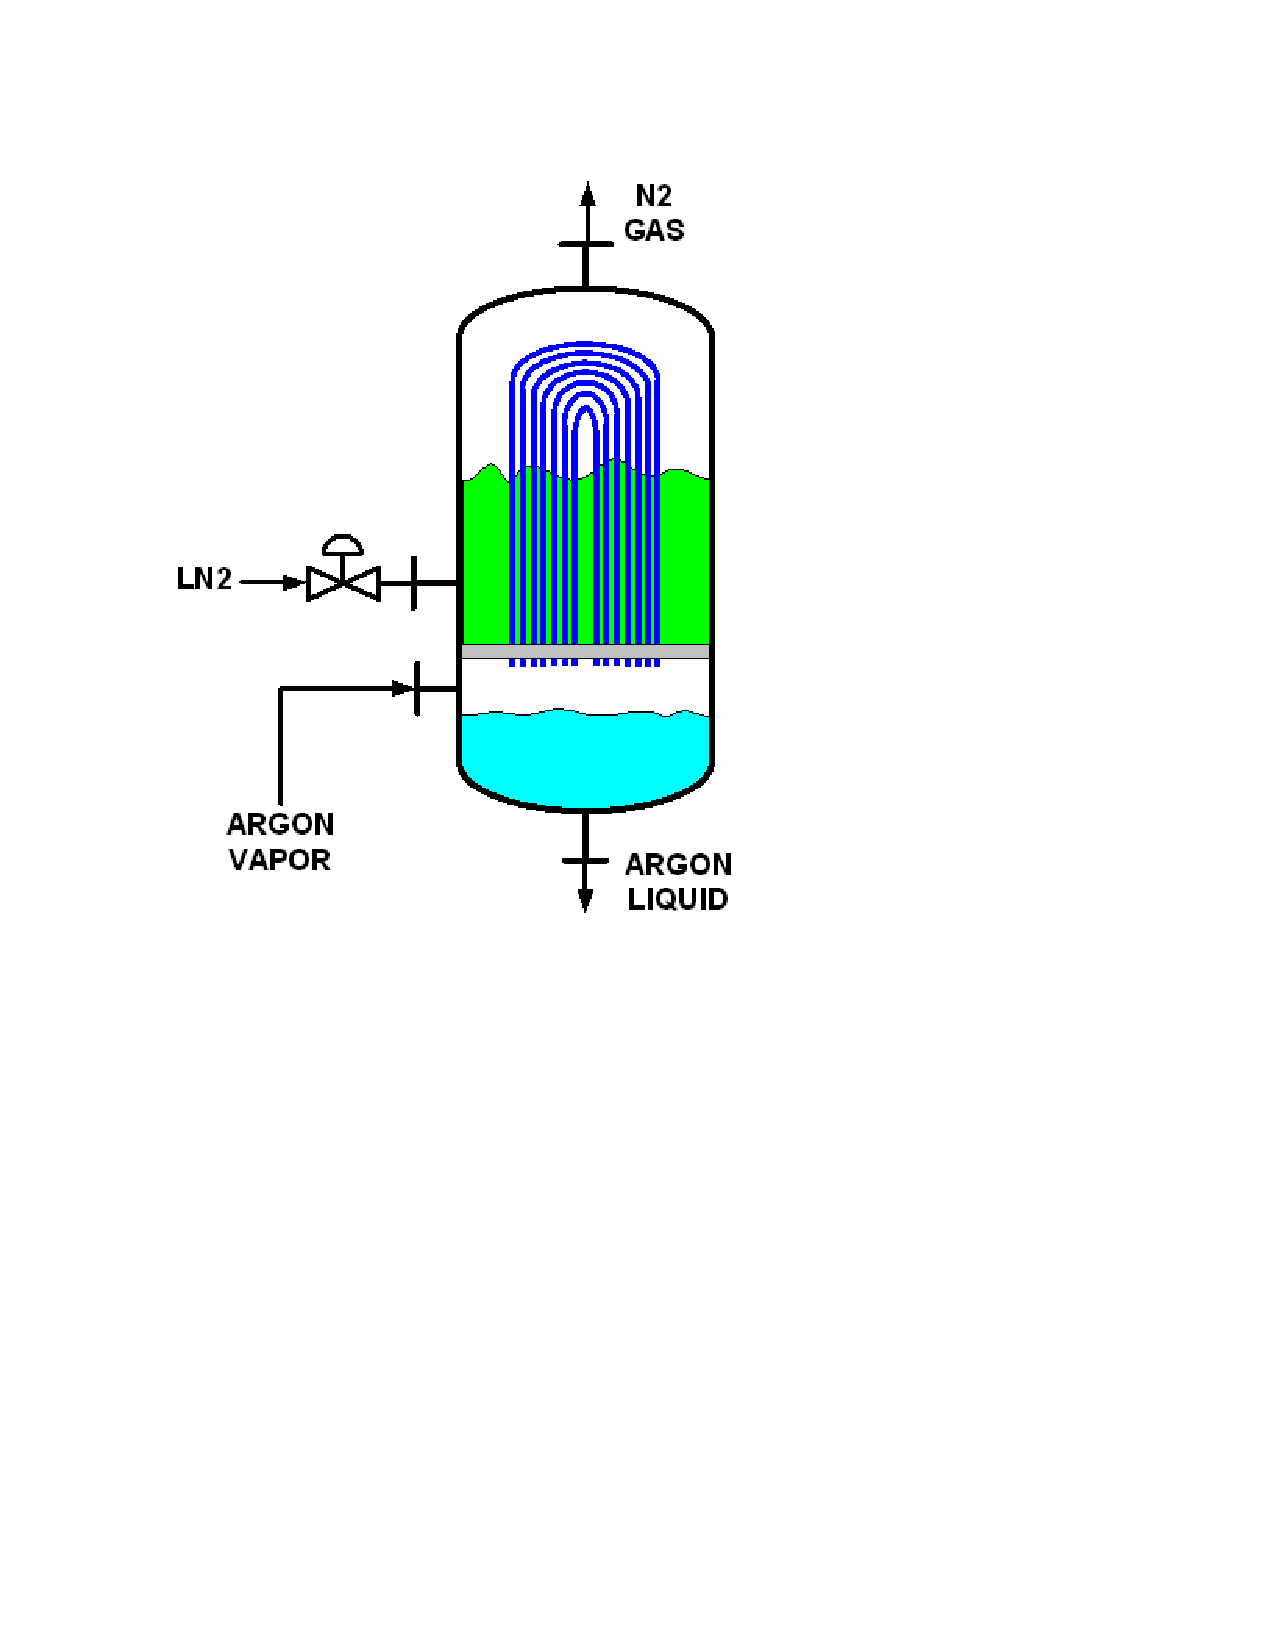
\includegraphics[width=.6\textwidth]{v5ch2-recondensor-2011}
\caption{Liquid argon recondenser}
\label{fig:v5ch2-recondenser-sept-2011}
\end{figure}

Each module of the detector has a dedicated nitrogen-refrigeration plant 
 and a third and fourth plant will be on standby during normal operations. All four will be used
for the initial cooldown of the cryostats
because of the large volume of gas which must be cooled from 300K to liquid
argon temperature (87K). Further, each module will
have two 85-kW condensers to provide the
cooling power needed during initial cooldown and filling operations where warm GAr
is cooled and reliquefied to fill the cryostat.
After filling, only one condenser is needed with the
other providing redundancy.
This will ensure high availability of the recondensing system, minimize the need to vent high-purity argon and allow down-time for maintenance of
the recondensers and the refrigeration plants. 

\subsection{Argon Purification}
\label{subsec:argon-pur}
Since the tank is designed without penetrations below the liquid level, pumps must be used to transfer LAr from the cryostat.  Vertical submersible 
pumps (see Figure~\ref{fig:vert-submers-pumps}) will be inserted into pump wells extending down from the cryostat roof.  The pump suction 
must be located a minimum distance (normally $\sim$1.5 to 2~m) below 
the lowest liquid level at which they are to pump in order to prevent cavitation and vapour-entrapment. 
The pumps and pump wells will extend to the bottom of the cryostat.  They 
could also be staggered at different elevations to allow flexibility in drawing liquid from different 
elevations. Vertical, submersible, cryogenic pumps are supplied by manufacturers such as Ebara and 
Carter Cryogenic Products.


\begin{figure}[htbp]
\centering
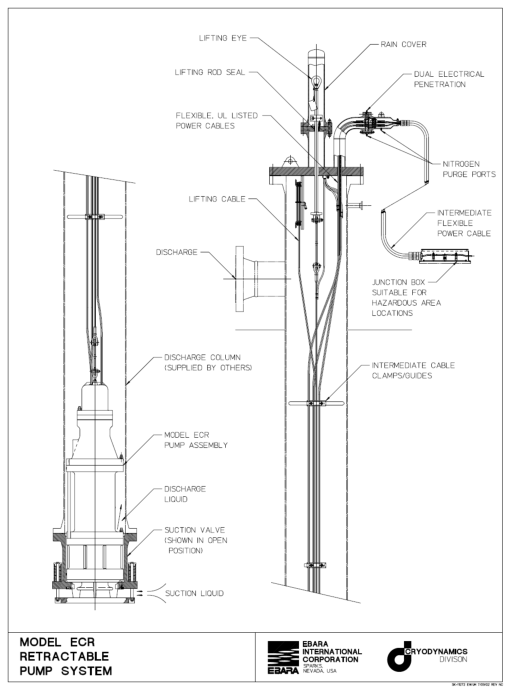
\includegraphics[width=.9\textwidth]{v5ch2-vert-submers-pumps}
\caption{Vertical submersible pump }
\label{fig:vert-submers-pumps}
\end{figure}

The required flow rate of liquid argon to be sent for purification is expected to decrease over time.  The 
initial maximum flow rate will be 51~m$^3$/hr (224~gpm).  The liquid-argon volume in one cryostat will turn over every five days at this rate. 
 Longer term, the rate will decrease to 25~m$^3$/hr with a turn-over rate of 11 days.  As a point of comparison, ICARUS T600 has a maximum turn-over rate of eight to ten days. See the table in Figure~\ref{fig:table:purif-compare} for a comparison of purification rates among other  experiments and LBNE. To achieve the turn-down required between the short- and long-term flow rates, two removable 25~m$^3$/hr (112~gpm) pumps will be located at the end of the cryostat.  Placing the pumps at this end of the cryostat will keep space clear for TPC installation. The purification skids are located at the 15~m wide septum which separates the two cryostats.  The multiple-pump arrangement will provide a very high level of redundancy, which will extend the maintenance-free operating period of the cryostat.  


The purification system consists of two filter vessels containing molecular-sieve and copper media filters. The filter is 2.4~m in diameter by 3.8~m tall. The filters are sized to provide effective media usage at low pressure drop (2~kPa or 0.3~psi) over the expected range of flow rates. 
One filter is for gas filtration during filling; the other is for liquid filtration. After filling is complete, the gas filter will be repurposed for liquid filtration.

The 
purifiers will be located close to the cryostat to minimize both the volume of LAr in the circulation pipework 
and the pump power required to achieve the desired flow rate.  
The cryostat liquid argon inventory is circulated through a purification filter to achieve and maintain the required purity. The purification filter, containing molecular sieve media to remove water and copper media to remove oxygen, will become saturated.
The nearly saturated purification filter is regenerated to vent the contaminants. The liquid argon flow is switched to another purification filter for uninterrupted filtration. 

A purity monitor after the purification filter will monitor the filter effectiveness. (Purity monitors measuring electron lifetime will also be in the LAr bath and resident in the cryostat.  It is a requirement that purity levels reach < 200 ppt oxygen equivalent to match the required electron lifetime of the detector). 

The regeneration of a filter is done in several steps. A saturated purification filter is first warmed with heated argon gas to an elevated temperature driving the captured water into the gas. Hydrogen gas is generated and mixed with the circulating argon gas up to 1.5\% hydrogen by volume. The hydrogen reacts with the oxygen and makes water that is also released into the circulating argon gas.
Argon gas is vented to purge water from the hot circulating gas. 

The hot filter full of regenerated media is cooled by circulating chilled argon gas. The circulating argon gas is chilled first with a heat exchanger using a commercial R-404A refrigeration unit until the filter is cold. The commercial refrigeration unit accumulates the R-404A liquid and shuts down. The filter is next cooled down to cryogenic temperatures by circulating argon gas chilled by a second heat exchanger with a liquid nitrogen coolant. This completes the regeneration steps for a purification filter. The filter is now ready to be switched into service or held cold until needed. Two spare purification filters are used with separate heating and cooling loops to reduce the usage rate of electricity and liquid nitrogen. This also reduces the stresses on heat exchangers by decreasing their temperature swings.


\begin{figure}[htbp]
\centering
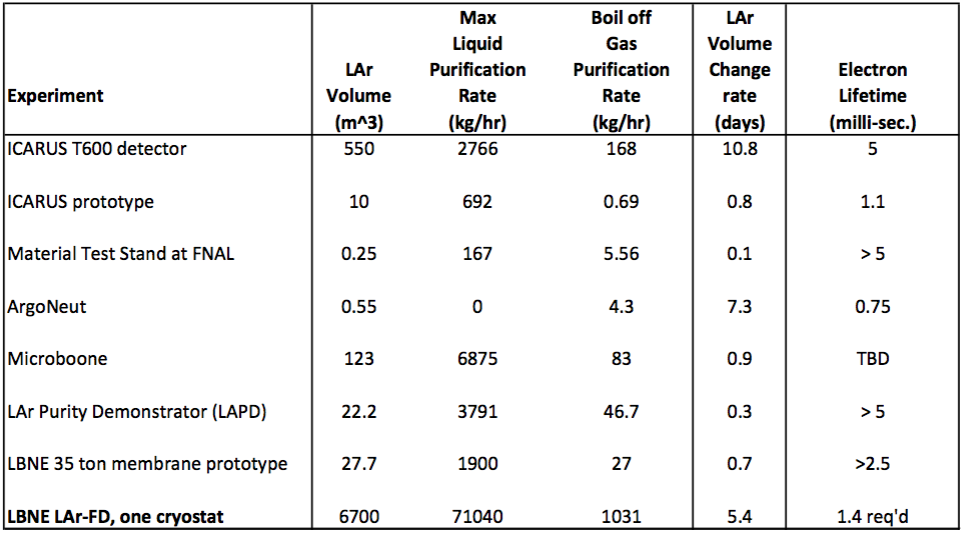
\includegraphics[width=.9\textwidth]{purification-comp-data-dec2014.png}
\caption{Purification comparision data for LArTPCs}
\label{fig:table:purif-compare}
\end{figure}

\subsection{Pressure Control}
\label{sec:press-control}

\subsubsection{Normal Operations}

The pressure-control valves are sized and set to control the internal cryostat pressure under normal operating conditions to the nominal design pressure of 0.113~MPa.  Fluctuations within the range 0.105~MPa (50~mbarg) to 0.120~MPa (200~mbarg) will be allowed.
%\fixme{note to self: put this unit in list of abbrevs}).  
Ten percent excursions above or below these levels will set off alarms to alert the operator to 
intervene.  Further excursion may result in automatic (executive) actions.  These actions may 
include stopping the LAr circulation pumps (to reduce the heat ingress to the cryostat), increasing the 
argon flow rate through the recondenser, increasing the LN$_2$ flow through the recondenser vessel, 
powering down heat sources within the cryostat (e.g., detector electronics).  Eventually, if the pressure continues to rise, it will trigger the pressure-relief valves to operate. Table~\ref{table:pressure-values} gives important pressure values.

%%%%%%%%%
\begin{table}
\centering
%\begin{tabular}[htbp]{| p{0.3\textwidth}|p{0.3\textwidth}||p{0.3\textwidth}|}
\caption{Important Pressure Values}
\label{table:pressure-values}\begin{tabular}[htbp]{|l|l|}
\hline 
Vessel ullage maximum operating pressure & 0.121 MPa, 200 mbarg, 2.9 psig\\
\hline
Relief valve set pressure& 0.125 MPa, 250 mbarg, 3.5 psig\\
\hline
Roof truss design working pressure& 0.135 MPa, 350 mbarg, 5.1 psig\\
\hline
\end{tabular} 

\end{table}
%%%%%%%%%

The ability of the control system to maintain a set pressure is dependent on the size of pressure upsets (due to changes in flow, heat load, temperature, atmospheric pressure, etc.) and the volume of gas in the system.  The reference design has 0.8 meters of gas at the top of the cryostat.  This is 5\% of the total argon volume and is the typical vapor fraction used for cryogenic storage vessels.  Reaction time to changes in the heat load is slow, on the order of an hour.  At the expected heat-load rate of 52.6~kW, and for an isolated or un-cooled cryostat, the rate of pressure rise would be 168~mbar (2.43 psi) per hour. 
We plan to provide two redundant pressure control valves to maintain the required pressure range, each sized to handle at least 7700 kg/hr of argon flow to the recondenser to handle the cooling and
reliquefaction of warm GAr during cryostat filling.


\subsubsection{Overpressure Control}

In addition to the normal-operation pressure-control system, it is planned to provide a cryostat overpressure-protection system.  This will need to be a high-integrity, automatic, failsafe system capable of preventing catastrophic structural failure of the cryostat in the case of excessive internal pressure.

The key active components of the planned system are pressure-relief valves (PRVs) located on the roof of the cryostat that will monitor the differential pressure between the inside and the outside of the cryostat and open rapidly when the 
differential pressure exceeds a preset value. 
 A pressure-sensing line is used to trigger a pilot valve which in turn opens the PRV.
A pressurized reservoir of power fluid is provided to each valve to ensure that the valves will operate under all upset and/or shutdown scenarios.  The PRVs are self-contained devices provided specially for tank protection; they are not normally part of the control system. 

The installation of the PRVs will ensure that each valve can periodically be isolated and tested for correct operation.  The valves must be removable from service for maintenance 
or replacement without impacting the overall containment envelope of the cryostat or the integrity of the 
over-pressure protection system.  This normally requires the inclusion of isolation valves upstream and downstream of the pressure-relief valves and at least one spare installed relief valve ($n+1$ provision).

When the valves open, argon is released, the pressure within the cryostat falls and argon gas discharges into the argon vent riser.  The valves are designed to close when the pressure returns below the preset level.

\subsubsection{Vacuum-Relief System}

The cryostat vacuum-relief system is a high-integrity, automatic, failsafe system designed to prevent catastrophic structural failure of the cryostat due to low internal pressure.  The vacuum-relief system protects the primary membrane tank. Activation of this system is a non-routine operation and is not anticipated to occur during the life of the cryostat. 

%Theoretically, 
Potential causes of reduced pressure in the cryostat include operation of discharge pumps while the liquid-return inlet valves are shut, gaseous argon condensing in the recondenser (a thermo-siphon effect) or a failure of the vent system when draining the cryostat.  Vacuum-relief valves are provided on LNG/LPG storage tanks to protect the structure from these types of events.  


%A vacuum relief system will be provided in addition to the normal pressure-control system.   
The key active components of this additional protection system are vacuum-relief valves located on the roof of the cryostat that will monitor the differential pressure between the inside and the outside of the cryostat and open when the differential pressure exceeds a preset value, allowing cavern air to enter the cryostat to restore a safe pressure. 

\subsection{LN$_2$ Refrigeration System}
\label{sec:ln-refrig-sys}
%BN modified refrigeration size 10/6/2011
Four commercial LN$_2$-refrigeration plants will be procured for LAr-FD.  After achieving the
required purity and completing initial fill, each cryostat will
have a dedicated LN$_2$ plant for steady-state operations.
The third and fourth plants will be used when the 30-kton detector is online. The plants will be located in the cavern in the 4850L configuration. Each will be a
closed-loop system supplying LN$_2$
to the argon recondenser. The nominal rating of the quoted
refrigerators is in the range of 85 kW.

Two-phase nitrogen is delivered from the cold end of the refrigerator into a farm of  LN$_2$ storage vessels with a total capacity of 50 m$^3$. Pure liquid is withdrawn from the  LN$_2$ storage vessels and is supplied via transfer line to a pressure-reducing valve and phase-separator tank also located within the cavern.  LN$_2$ is then withdrawn from the bottom of the phase-separator tank, at a pressure of 2.0 bar and temperature of 84K, and directed to the recondenser. This results in a 5K temperature difference relative to the 89K argon recondenser temperature. The eight 12.5 m$^3$ LN$_2$ vessels will allow for greater than forty hours of refrigeration time. This time window is adequate to cover most power outages, refrigerator performance problems and refrigerator switch-overs.



The refrigeration system operation, illustrated in Figure~\ref{fig:LN2-refrigerator-flow}, is based on a screw compressor package and three turbo expanders. This system is expected to be capable of running  
continuously for at least a year, and then require only minor servicing. The system will be equipped with 
automatic controls and a remote monitoring so that no operator will be required during normal operation. 
Estimated maximum power requirement is 850 hp (650 kVA) , not taking into account the power generated by the expanders.  The LAr-FD reference design places the nitrogen compressor  in a surface-level equipment building. A closed-loop water system with evaporative-cooling tower removes heat from the compressor. Compression is carried out at close-to-ambient temperature. A compressor aftercooler is provided to reject heat. 

\begin{figure}[htbp]
\centering
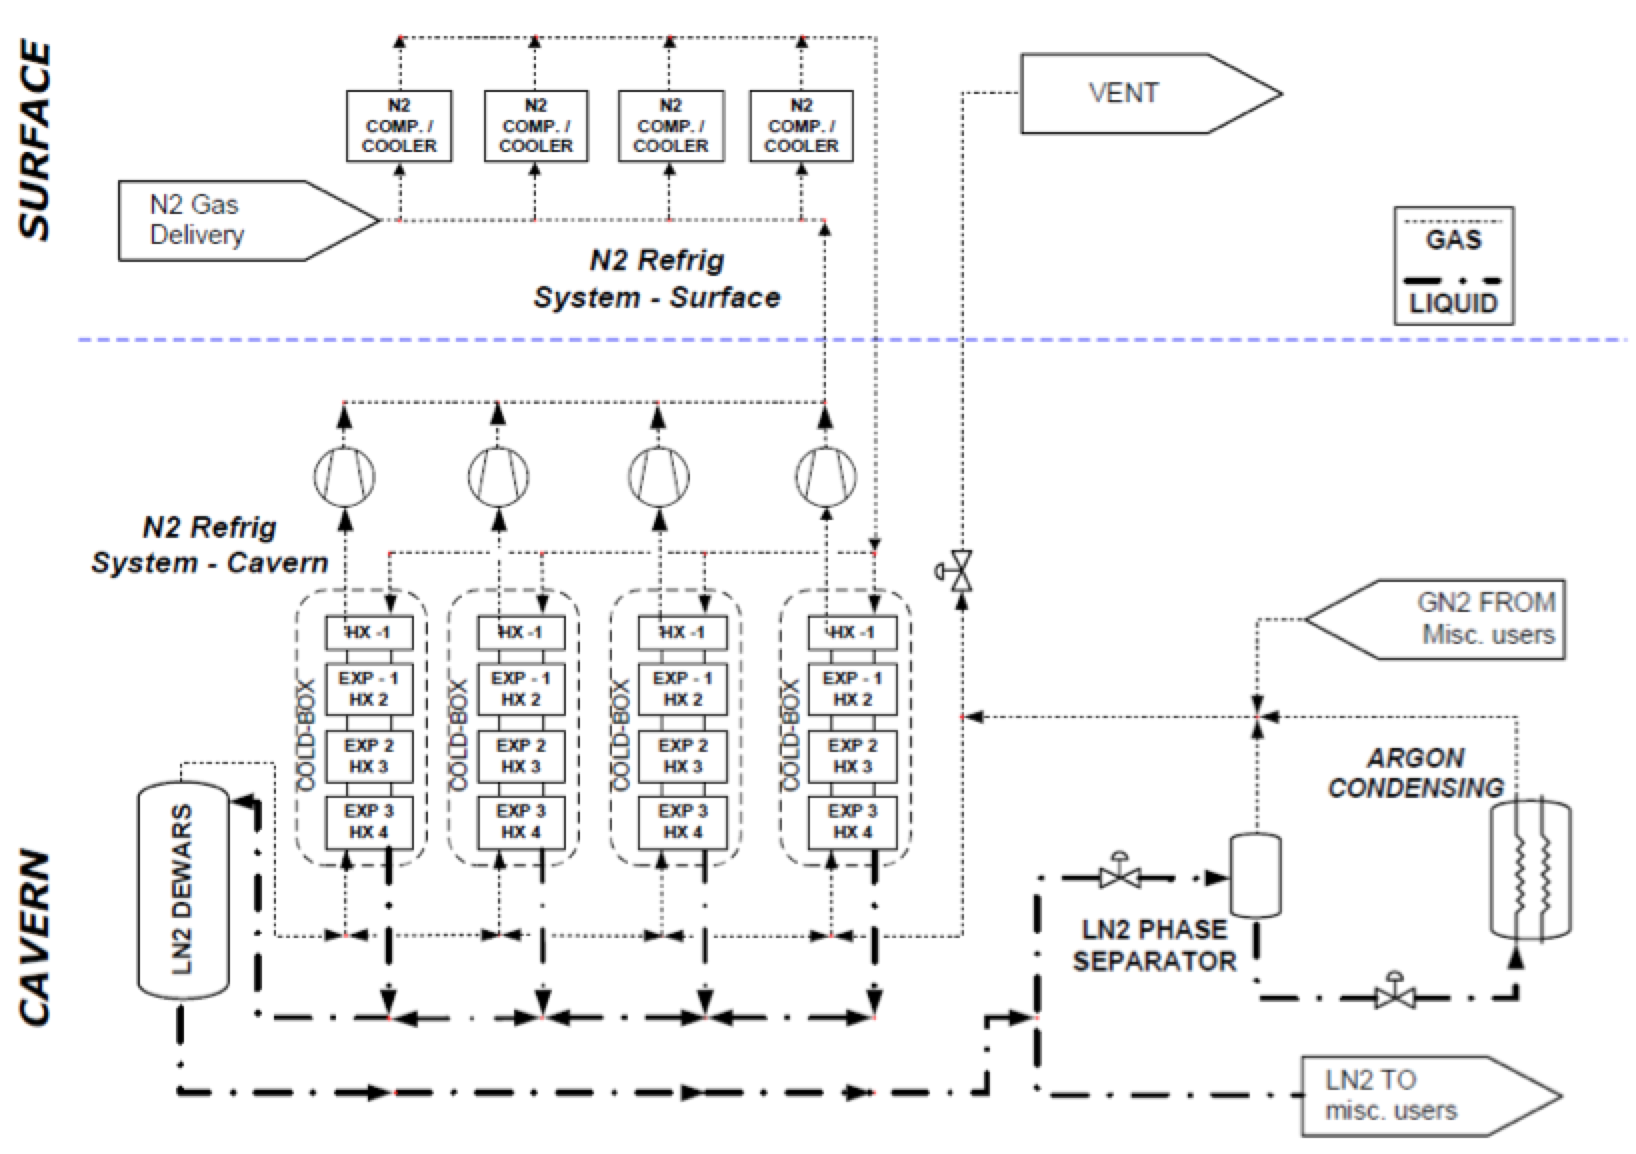
\includegraphics[%scale=1.2
width=.7\textwidth]{nitrogen-refrig-plant-flow.png}
\caption{Nitrogen refrigeration-plant flow diagram}
\label{fig:LN2-refrigerator-flow}
\end{figure}

The fluid is next routed to a `cold box' consisting of four heat exchangers.  This series of exchangers provides staged heat transfer from a cooling nitrogen stream to a warming one.  The expanders are connected between the heat exchangers to progressively reduce the pressure of the cooling nitrogen stream to isentropically reduce the pressure and temperature of the
nitrogen stream, eventually leading to a large liquid-nitrogen fraction at the coldest end of the cold box. 

The main cold box shell is 1.22~m (4~ft) in diameter and 8.2~m (27~ft) tall, as illustrated in
Figure~\ref{fig:nitrogren-refrigerator}.  The expanders are adjacent to the cold box at three elevations and extend about 1~m to the side of the cold-box shell.  The cold box will weigh 5670~kg. The compressors are located at the surface inside an equipment shed. The compressor skid (frame) is 4.3~m long, 1.8~m wide and 2.7~m tall and will weigh approximately 3630~kg.  

\begin{figure}[htbp]
\centering
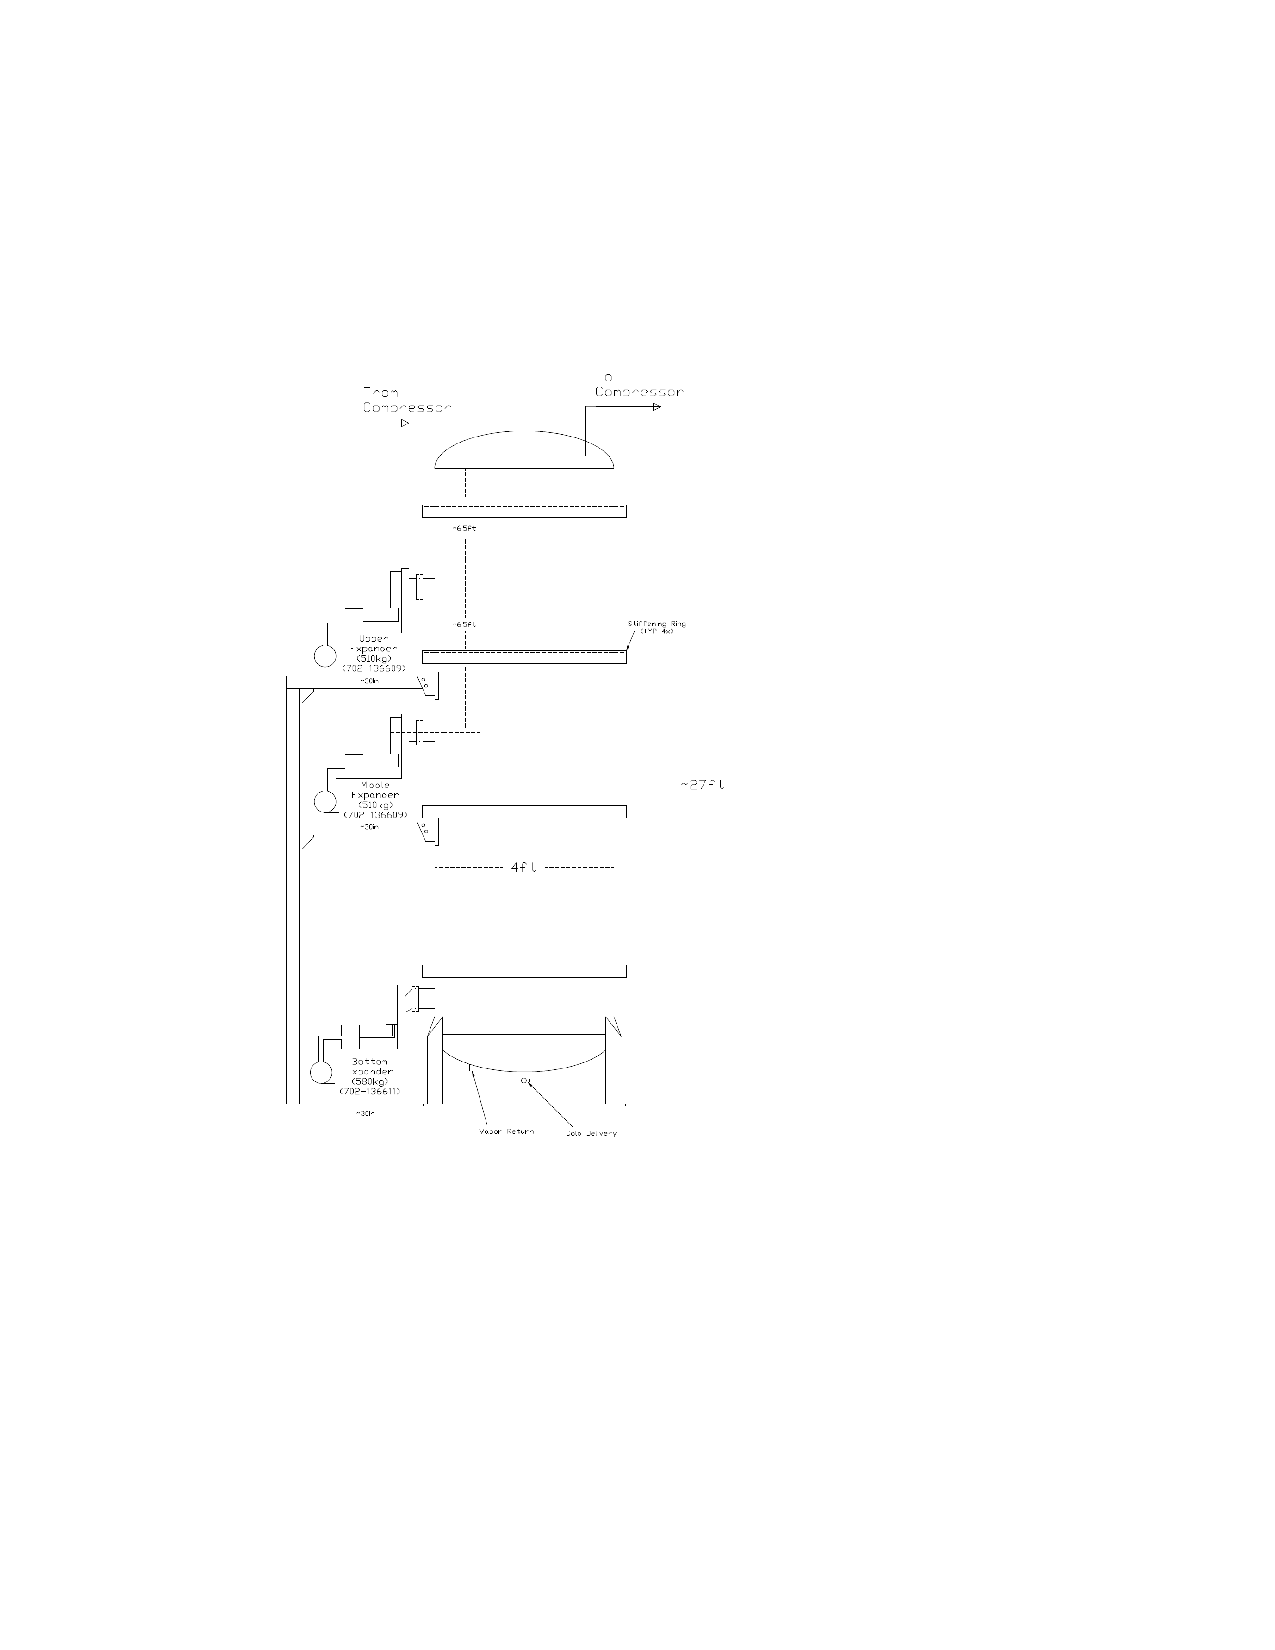
\includegraphics[width=.6\textwidth]{v5ch2refrigplant}
\caption{Nitrogen refrigeration plant}
\label{fig:nitrogren-refrigerator}
\end{figure}

\subsection{Refrigeration Load Scenarios}

\begin{editornote}
  Editor's Note:  The load scenario information contained in this section is relevant for a 34-kton fiducial mass detector made up of two 17-kton modules.  As of late 2014, the refrigerator will need to serve the first 10-kton detector cavern and the 30-kt detector cavern.
\end{editornote}

In order to determine the optimal plant capacity and number of plants required, we forecast the LN$_2$ refrigeration loads and plant capacity needed over seven scenarios.  Those scenarios are described below and a summary table is shown in Figure~\ref{fig:Refrigeration-loads}. 

The conclusion points to the requirement of four 85-kW plants.  Each of these plants can achieve a 20\% turn up or turn down.  Scenario 1 and 4 impose the most severe requirements. In this scenario, all four plants will be required to operate at a duty cycle of approximately 85\%. This scenario includes one completely filled and purified cryostat while the second is being purified and requiring frequent filter regeneration.

\begin{description}
\item[Scenario 1]
The initial operation will be the purging, cooling and filling of the first cryostat, condensing gaseous argon in the cavern by heat exchange via the recondensers.
The surface and cavern LAr and  LN$_2$ dewars will be operational and the cooling load for the
dewars will come directly from the refrigeration plant. The cavern pipework and vessels will
be cold, the LAr in the cryostat will be circulating at high flow rate through the
purification plant, and the cryostat will be cold.  The cryostat cool-down rate is constrained by three variables: 1) The size of the piping from the surface to bottom of Ross Shaft, 2) The size of the LN$_2$ refrigeration units, and 3) the cooling power available via the recondensers.  All three variables have been matched for the physical constraints of a 34 kton module at 4850 using the Ross shaft. The refrigerators and condensers have been sized to accommodate the long-term refrigeration load associated with the cryostats.  As the LAr is circulated to achieve the operational purity the filtration plant will need to be regularly regenerated. This will mean that the associated refrigeration load will normally be present.


\item[Scenario 2]
Once the first cryostat is filled with LAr the cool-down load will reduce to zero and the cryogenic plant will run for several months purifying the LAr inventory.

\item[Scenario 3]
When the LAr in the cryostat reaches the required purity level, the circulation flow rate will be reduced and the detector electronics will be turned on.  At this stage the recondenser refrigeration load falls such that only one recondenser is required and the second and third units can operate as spare units.

\item[Scenario 4] The first cryostat continues to operate in normal experimental mode %and
while  the second cryostat is being purged, cooled down and filled with LAr. Again a very large burden is placed on the recondensers due to the gas condensation and rate of liquification.

\item[Scenario 5] The second cryostat is full and LAr is circulated at high flowrate through the purification plant.  The first cryostat continues to operate as normally.

\item[Scenario 6]
Both cryostats are operating in normal experimental mode.  A spare recondenser is available on each cryostat to facilitate maintenance.

\item[Scenario 7]
It is assumed that a total failure of the refrigeration plant has occurred. All noncritical heat sources are isolated and liquid nitrogen from the cavern LN$_2$ vessels is utilized to recondense the inventory of high purity LAr. Nitrogen refrigeration must be reestablished before the liquid nitrogen reservoir is exhausted or the high purity argon will need to be vented. In the locked-down state the circulation pumps and the purification plants are shut down.
\end{description}

\begin{figure}[htbp]
\centering
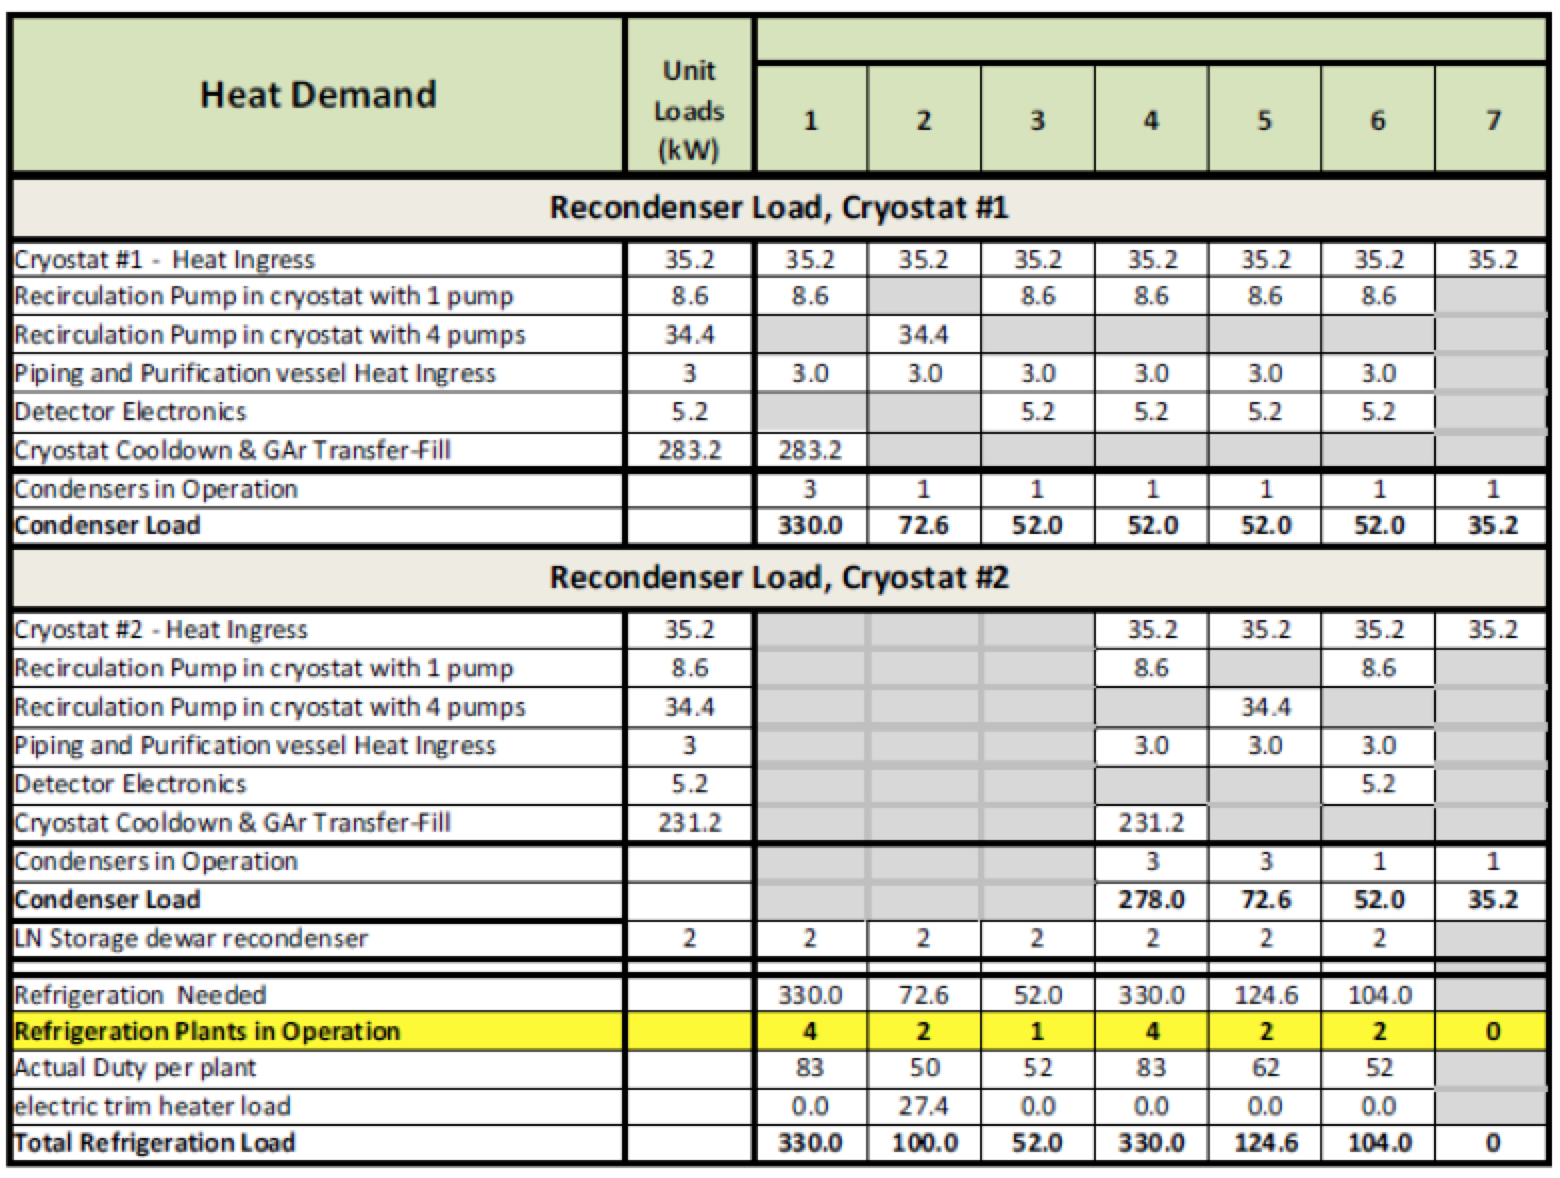
\includegraphics[width=\textwidth, angle = 90]{refrig-loads.png}
\caption{Refrigeration loads}
\label{fig:Refrigeration-loads}
\end{figure}

\begin{figure}[htbp]
\centering
%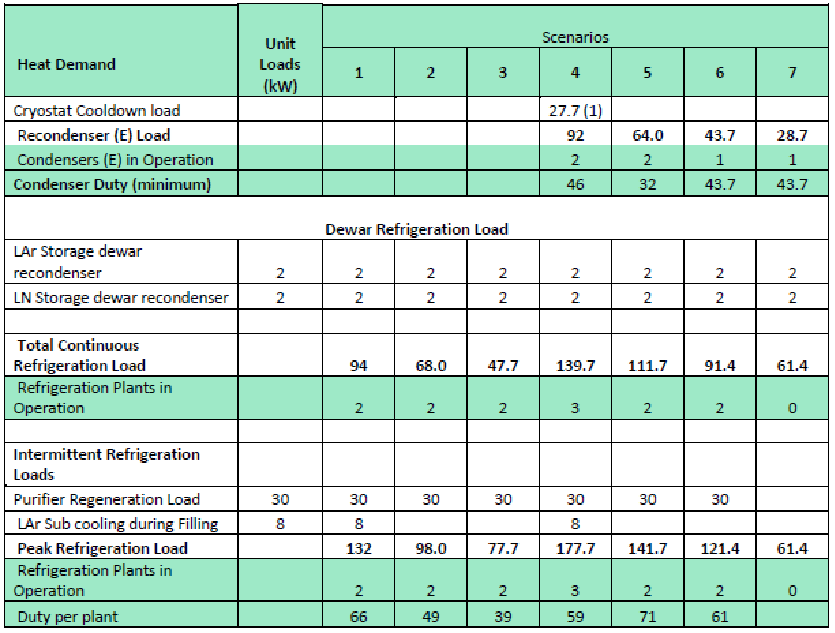
\includegraphics[scale=1, angle = 90]{v5ch2-arup-refrigeration-loads-fig2}
%\caption{Refrigeration loads, continued}
%\label{fig:Refrigeratior-loads-2}
\end{figure}


\section{Prototyping Plans}
\label{sec:cryo-cryosys-proto-plans}

\begin{editornote}
  Editor's Note:  LAPD has successfully achieved greater than 5 millisecond electron lifetime, and the LBNE 35t has also achieved greater than 2.5 milli-second electron lifetime. 
\end{editornote}

The development of the LAr-FD from conceptual to preliminary design will include a prototyping program. The most significant issue to resolve is whether a membrane cryostat the size of LAr-FD can achieve the required electron-drift lifetime. The Liquid Argon Purity Demonstrator (LAPD), already in progress and introduced in Section~\ref{sec:lapd}, is an off-project prototype being built as part of a development program at Fermilab to study the scaling of LArTPCs to kiloton sizes. In addition, a 35-ton membrane-cryostat prototype is being developed as an LBNE effort to confirm, among other things, that at larger scales the required LAr purity can still be achieved. It is scheduled for initial operation in late summer 2013. The prototype will be used to repeat the purge process accomplished in the LAPD to confirm that initial evacuation of the cryostat is unnecessary. This work will also seek to confirm that an LAr purity level sufficient to enable the required drift times in a membrane cryostat can be achieved.



\section{ES\&H}
\label{sec:cryo-cryosys-esh}

During all phases of LAr-FD and the proposed protoypes, Fermilab ES\&H standards and
Sanford Laboratory ES\&H codes and standards will guide the design, procurement and
installation phases of the project. Particular attention will be paid to critical sections of
Chapter 5000~\cite{feshm} relating to ODH, standards for piping construction and vessel design. The
planned work process will provide for reviews throughout all phases of the project to guarantee
stringent adherence to the safety requirements. Requirements on the membrane-cryostat
materials and their fabrication will be strictly outlined in the specification documents. Close
communication between the vendors, Fermilab's cryogenic and process engineers, and Fermilab and Sanford Laboratory ES\&H personnel will be maintained at all times.
